\documentclass[12pt,a4paper]{article}
\usepackage[utf8]{inputenc}
\usepackage{vietnam}
\usepackage[left=3cm, right=2cm, top=2.5cm, bottom=2.5cm]{geometry}
\usepackage{amsmath}
%\usepackage{asmfonts}
\usepackage{float}
\usepackage{amssymb}
\usepackage{multirow} 
\usepackage{graphicx} % thư viện hiển thị hình ảnh
\usepackage[hidelinks, unicode]{hyperref} % thư viện link tới chương
\usepackage{caption} % thư viện đặt caption
\usepackage[table]{xcolor} % thư viện hiển thị màu cho bảng
%\usepackage{indentfirst}
\usepackage{mathptmx} % thư viện times new roman
\usepackage{booktabs,tabularx} %thư viện bảng sách
\usepackage{courier}
\newcommand{\code}[1]{\texttt{#1}}

\renewcommand{\baselinestretch}{1.5}

\newcommand{\subsubsubsection}[1]{\paragraph{#1}\mbox{}\\}

\setcounter{secnumdepth}{4}
\setcounter{tocdepth}{4}
\geometry{letterpaper}
\title{\textbf{ĐỒ ÁN KHAI THÁC}}
\author{Truong Manh Phi\\Bui Trong Nghia}

\begin{document}

\pagenumbering{gobble}
%\thispagestyle{empty}
\clearpage

\pdfbookmark{\contentsname}{content}
\maketitle

\newpage
\begin{center}
	\centering
	\text{ĐỒ ÁN ĐƯỢC HOÀN THÀNH TẠI}\\ 
	\textbf{TRƯỜNG ĐẠI HỌC DẦU KHÍ VIỆT NAM}
\end{center}
Người hướng dẫn chính:..................................................\\
(\textit{Ghi rõ họ, tên, học hàm, học vị})\\
\newline
Người hướng dẫn phụ (\textit{Nếu có}):......................................\\
(\textit{Ghi rõ họ, tên, học hàm, học vị})\\
\newline
Người chấm phản biện:....................................................\\
(\textit{Ghi rõ họ, tên, học hàm, học vị})\\
\newline
\newline
\newline
\newline
\newline
\newline
Đồ án được bảo vệ tại:
\begin{center}
	\centering
	\textbf{HỘI ĐỒNG CHẤM ĐỒ ÁN MÔN HỌC}\\
	\textbf{TRƯỜNG ĐẠI HỌC DẦU KHÍ VIỆT NAM}\\
	Ngày .... tháng .... năm ....
\end{center}
\newpage
\begin{table}[h]
\centering
\label{my-label}
\begin{tabular}{cc}
 \textbf{TRƯỜNG ĐẠI HỌC DẦU KHÍ VIỆT NAM} & \textbf{CỘNG HÒA XÃ HỘI CHỦ NGHĨA VIỆT NAM} \\
 \underline{\textbf{KHOA DẦU KHÍ}}& \underline{\textbf{ĐỘC LẬP - TỰ DO - HẠNH PHÚC}}
\end{tabular}
\end{table}
\begin{center}
	\centering
	\textbf{NHIỆM VỤ ĐỒ ÁN MÔN HỌC}
\end{center}

\textbf{Họ và tên SV:} \textit{Bùi Trọng Nghĩa} \hspace{98pt} \textbf{MSSV:} \textit{04PET110011} 

\hspace{68pt} \textit{Trương Mạnh Phi} \hspace{95pt} \textbf{MSSV:} \textit{04PET110014}

%\hspace{68pt} \textit{Vũ Thành Hiếu} \hspace{114pt} \textbf{MSSV:} \textit{04PET110007} \par
\textbf{Ngành:} \textit{Kỹ thuật dầu khí} \hspace{130pt} \textbf{Lớp:} \textit{K4KKT}
\begin{enumerate}
	\item Tên đồ án môn học: \textit{Nghiên cứu tối ưu hóa tỉ số độ linh động trong thu hồi dầu tăng cường bằng phương pháp polymer sử dụng mô hình sandpack.}
	\item Nhiệm vụ(Nội dung đồ án):\\
	- Tìm hiểu tổng quan về thu hồi dầu tăng cường\\
	- Tìm hiểu tổng quan về phương pháp bơm ép polymer\\
	- Tìm hiểu các lý thuyết liên quan đến tính toán tối ưu tỉ số độ linh động\\
	- Tìm hiểu cơ bản về thí nghiệm sandpack\\
	- Tính toán tối ưu hóa tỉ số độ linh động thông qua đo đạt các thông số cần thiết bằng mô hình sandpack.
	\item Ngày giao đồ án môn học: \textit{13/03/2018}
	\item Ngày hoàn thành đồ án môn học: \textit{15/05/2018}
	\item Họ và tên người hướng dẫn: \textit{Ths. Phạm Hữu Tài}.	
\end{enumerate}
\begin{flushright}
Bà Rịa - Vũng Tàu, ngày \ldots tháng \ldots năm \ldots
\end{flushright}
\textbf{HIỆU TRƯỞNG} \hspace{30pt} \textbf{TRƯỞNG PHÒNG ĐÀO TẠO} \hspace{30pt} \textbf{NGƯỜI HƯỚNG DẪN}\\
(Ký, ghi rõ họ tên) \hspace{60pt} (Ký, ghi rõ họ tên) \hspace{80pt} (Ký, ghi rõ họ tên)
%\clearpage
\newpage
\begin{table}[h]
\centering
\label{my-label}
\begin{tabular}{cc}
 \textbf{TRƯỜNG ĐẠI HỌC DẦU KHÍ VIỆT NAM} & \textbf{CỘNG HÒA XÃ HỘI CHỦ NGHĨA VIỆT NAM} \\
 \underline{\textbf{KHOA DẦU KHÍ}}& \underline{\textbf{ĐỘC LẬP - TỰ DO - HẠNH PHÚC}}
\end{tabular}
\end{table}
\begin{center}
	\centering
	\textbf{PHIẾU NHẬN XÉT ĐỒ ÁN MÔN HỌC}\\
	(Mẫu dành cho người hướng dẫn)
\end{center}
\textbf{Tên đề tài:} Nghiên cứu tối ưu hóa tỉ số độ linh động trong thu hồi dầu tăng cường bằng phương pháp polymer sử dụng mô hình sandpack.\\
\textbf{Họ và tên người hướng dẫn:} \textit{Ths. Phạm Hữu Tài}.

\textbf{Họ và tên SV:} \textit{Bùi Trọng Nghĩa} \hspace{98pt} \textbf{MSSV:} \textit{04PET110011} 

\hspace{68pt} \textit{Trương Mạnh Phi} \hspace{95pt} \textbf{MSSV:} \textit{04PET110014}

%\hspace{68pt} \textit{Vũ Thành Hiếu} \hspace{114pt} \textbf{MSSV:} \textit{04PET110007} \par
\textbf{Ngành:} \textit{Kỹ thuật dầu khí} \hspace{130pt} \textbf{Lớp:} \textit{K4KKT}
\begin{enumerate}
	\item Nhận xét về tinh thần và thái độ làm việc của sinh viên: .................................................\\...........................................................................................................................................\\...........................................................................................................................................
	\item Nhận xét về kết quả đạt được: .........................................................................................\\..........................................................................................................................................\\..........................................................................................................................................
	\item Những điểm thiếu xót còn tồn tại: ...................................................................................\\..........................................................................................................................................\\..........................................................................................................................................
\end{enumerate}
\begin{flushright}
Bà Rịa - Vũng Tàu, ngày \ldots tháng \ldots năm \ldots \\
\end{flushright}
\hspace{300pt} \textbf{NGƯỜI HƯỚNG DẪN}\\
\hspace*{316pt} (Ký, ghi rõ họ tên)

\newpage
\begin{table}[h]
\centering
\label{my-label}
\begin{tabular}{cc}
 \textbf{TRƯỜNG ĐẠI HỌC DẦU KHÍ VIỆT NAM} & \textbf{CỘNG HÒA XÃ HỘI CHỦ NGHĨA VIỆT NAM} \\
 \underline{\textbf{KHOA DẦU KHÍ}}& \underline{\textbf{ĐỘC LẬP - TỰ DO - HẠNH PHÚC}}
\end{tabular}
\end{table}
\begin{center}
	\centering
	\textbf{PHIẾU NHẬN XÉT ĐỒ ÁN MÔN HỌC}\\
	(Mẫu dành cho người phản biện)
\end{center}
\textbf{Tên đề tài:} Nghiên cứu tối ưu hóa tỉ số độ linh động trong thu hồi dầu tăng cường bằng phương pháp polymer sử dụng mô hình sandpack.\\
\textbf{Họ và tên người hướng dẫn:} \textit{Ths. Phạm Hữu Tài}.

\textbf{Họ và tên SV:} \textit{Bùi Trọng Nghĩa} \hspace{98pt} \textbf{MSSV:} \textit{04PET110011} 

\hspace{68pt} \textit{Trương Mạnh Phi} \hspace{95pt} \textbf{MSSV:} \textit{04PET110014}

%\hspace{68pt} \textit{Vũ Thành Hiếu} \hspace{114pt} \textbf{MSSV:} \textit{04PET110007} \par
\textbf{Ngành:} \textit{Kỹ thuật dầu khí} \hspace{130pt} \textbf{Lớp:} \textit{K4KKT}
\\ \textbf{Phần nhận xét:}
\begin{enumerate}
	\item Về hình thức và kết cấu đồ án môn học: ........................................................................\\........................................................................................................................................
	\item Về nội dung: ..................................................................................................................\\........................................................................................................................................\\........................................................................................................................................\\........................................................................................................................................\\........................................................................................................................................
\end{enumerate}
\textbf{Điểm:}....................................................(Ghi bằng chữ)
\begin{flushright}
Bà Rịa - Vũng Tàu, ngày \ldots tháng \ldots năm \ldots \\
\end{flushright}
\hspace{300pt} \textbf{NGƯỜI PHẢN BIỆN}\\
\hspace*{310pt} (Ký, ghi rõ họ tên)
\newpage
\begin{center}
	\centering
	\textbf{LỜI CAM KẾT}
	%\section*{\textbf{LỜI CAM KẾT}}
	\addcontentsline{toc}{section}{LỜI CAM KẾT}
\end{center}
Chúng tôi xin cam đoan những kết quả nghiên cứu được trình bày trong đồ án này là hoàn toàn trung thực, không vi phạm bất cứ điều gì trong luật sở hữu trí tuệ và pháp luật Việt Nam. Nếu sai, chúng tôi sẽ hoàn toàn chịu trách nhiệm trước pháp luật.\\
\hspace*{250pt} \textbf{ĐẠI DIỆN TÁC GIẢ ĐỒ ÁN}\\
\hspace*{280pt} (Ký, ghi rõ họ tên)
\newline
\newline
\hspace*{282pt} \textit{Bùi Trọng Nghĩa}


\clearpage
%\newpage

\pagenumbering{roman}
\thispagestyle{empty}
%\clearpage

\begin{center}
	\centering
	\textbf{LỜI CẢM ƠN}
	%\section*{\textbf{LỜI CẢM ƠN}}
	\addcontentsline{toc}{section}{LỜI CẢM ƠN}
\end{center}
Với lòng biết ơn sâu sắc nhất, nhóm em xin gửi đến quý Thầy Cô ở khoa Dầu Khí –
trường Đại Học Dầu Khí Việt Nam, không những dùng tri thức và tâm huyết của mình để truyền đạt vốn kiến thức quý báu cho chúng em trong suốt thời gian học tập tại trường mà còn tạo điều kiện và luôn ủng hộ nhóm em trong quá trình nghiên cứu hoàn thiện đồ án của nhóm. \\
Đồng thời chúng em xin gửi lời cám ơn chân thành đến thầy \textbf{Phạm Hữu Tài} đã đồng ý trở thành người trực tiếp hướng dẫn, đưa ra gợi ý và kịp thời chỉ ra những sai sót cho chúng em trong suốt thời gian hoàn thiện đồ án.\\
Qua quá trình hoàn thiện đồ án, nhóm đã có nhiều cơ hội với những kiến thức mới đồng thời cũng cố và vận dụng những kiến thức chuyên ngành vào thực tế, rèn luyện được kĩ năng nghiên cứu thực tế bổ ích từ thầy \textbf{Phạm Hữu Tài}.\\
Do mới bước đầu tiếp cận nghiên cứu đồ án cùng với lượng kiến thức còn hạn chế nên kết quả hoàn thiện còn nhiều thiếu sót. Kính mong quý Thầy, Cô đóng góp thêm ý kiến để những đồ án tiếp theo nhóm em có thể đạt kết quả tốt hơn và có thể hoàn thiện được bản thân mình hơn.
\begin{flushright}
Nhóm chúng em xin chân thành cảm ơn!
\end{flushright}

\newpage
\section*{\textbf{\LARGE Danh pháp và kí hiệu}}
\addcontentsline{toc}{section}{Danh pháp và kí hiệu}
\hspace*{1cm}\textbf{Danh pháp}
	\begin{enumerate}
		\item[] EOR \hspace*{50pt} Enhanced Oil Recovery
		\item[] OOIP \hspace*{45pt} Original Oil In Place
		\item[] HPAM \hspace*{39pt} Hydrolyzed Polyacrylamides
		\item[] KYPAM \hspace*{29pt} Salinity-Tolerant Polyacrylamides
		\item[] AMPS/AM \hspace*{15pt} 2-Acrylamide-2-Methyl Propane-Sulfonate Copolymer
		\item[] HEC \hspace*{47pt} Hydroxyethyl Cellulose
		\item[] HMSPAM \hspace*{19pt} Hydrophobically Modified Acrylamide-based Copolymer
		\item[] TPV \hspace*{47pt} Total Pore Volume
		\item[] OLS \hspace*{47pt} Ordinary Least Squares
		\item[] RSM \hspace*{44pt} Response Surface Methodology
	\end{enumerate}
	\newpage
	\noindent
\hspace*{1cm}\textbf{Kí hiệu}
	\begin{enumerate}
		\item[] $f_o$ \hspace*{50pt} Tốc độ dòng chảy tỉ đối
		\item[] M \hspace*{50pt} Tỉ số độ linh động 
		\item[] $q_o$ \hspace*{50pt} Lưu lượng dầu trong vỉa, $m^3/s$
		\item[] $q_w$ \hspace*{48pt} Lưu lượng nước trong vỉa, $m^3/s$
		\item[] $E_D$ \hspace*{46pt} Hiệu suất đẩy, \%
		\item[] $S_{oi}$ \hspace*{47pt} Độ bão hòa dầu ban đầu, \%
		\item[] $S_{or}$ \hspace*{47pt} Độ bão hòa dầu dư, \%
		\item[] $\lambda_D$ \hspace*{47pt} Độ linh động của pha chất lưu thay thế
		\item[] $\lambda_d$ \hspace*{50pt} Độ linh động của pha chất lưu bị thay thế
		\item[] OOIP \hspace*{34pt} Lượng dầu ban đầu, $cm^3$ 
		\item[] PV \hspace*{47pt} Thể tích nước bơm ép, $cm^3$
		\item[] $\phi$ \hspace*{54pt} Độ rỗng, \%
		\item[] $k_{ro}$ \hspace*{48pt} Độ thấm tương đối của dầu, mD
		\item[] $k_{rw}$ \hspace*{47pt} Độ thấm tương đối của nước, mD
		\item[] $S_{wD}$ \hspace*{45pt} Độ bão hòa của nước trong hệ hai độ rỗng, \%
		\item[] $S_{wi}$ \hspace*{50pt} Độ bão hòa nước ban đầu, \%
		\item[] $S_{or}$ \hspace*{50pt} Độ bão hòa dầu dư, \%
		\item[] $S_{orwf}$ \hspace*{39pt} Thể tích lượng dầu thu hồi, $cm^3$
	\end{enumerate}



\clearpage
\pagenumbering{arabic}
\newpage

\tableofcontents
\addcontentsline{toc}{section}{Mục lục}
\newpage

\listoftables
\addcontentsline{toc}{section}{Danh sách bảng}
\newpage

\listoffigures
\addcontentsline{toc}{section}{Danh sách hình}
\newpage

\section{Tổng quan}
Kể từ hơn một thế kỉ trước, con người đã phải phụ thuộc rất nhiều về nguồn năng lượng dầu mỏ, cách đây hơn nửa thế kỉ người Mỹ đã có thể khai thác dầu bằng công nghệ khoan. Trong nhiều năm qua, các chuyên gia về năng lượng đã dự báo về sự phụ thuộc của con người về nguồn nguyên liệu dầu mỏ và nhu cầu nhập khẩu dầu thô. Mặc dù có rất nhiều cường quốc về dầu mỏ trên thế giới nhưng theo thống kê các công ty dầu mỏ chỉ thu hồi được khoảng 32\% từ các mỏ dầu thông thường. Việc thu hồi được tất cả dầu trong vỉa là điều không thể nhưng tăng khả năng thu hồi dầu thì có thể, đó chính là mục tiêu để con người tiếp tục nghiên cứu phát triển các phương pháp có khả năng nâng cao lượng dầu khai thác được, góp phần vào đảm bảo an ninh năng lượng của mỗi quốc gia.\\
Hiện nay, các phương pháp khai thác dầu đang được sử không còn mang lại hiệu quả cao, sản lượng khai thác thấp, trữ lượng dầu trong vỉa được xác định còn lại khá nhiều. Điều đó thôi thúc các nhà khoa học tìm kiếm phương pháp và cách thức giúp duy trì năng lượng vỉa và thu hồi được nhiều dầu hơn. Tên của phương pháp này được gọi là phương pháp thu hồi dầu tăng cường “Enhanced Oil Recovery (EOR)”.\\
Hoạt động khai thác dầu được chia làm ba giai đoạn chính: Sơ cấp (primary) thứ cấp (secondary) và tam cấp (tertiary) \cite{green1998enhanced} theo vòng đời của giếng. Khai thác ở giai đoạn sơ cấp là hình thức khai thác tự phun dựa vào năng lượng ban đầu của vỉa với các cơ chế năng lượng vỉa khác nhau. Khi hình thức khai thác sơ cấp không còn mang lại hiệu quả cao, năng lượng vỉa bị sụt giảm làm cho năng suất sản lượng đi xuống thì bước vào khai thác ở giai đoạn thứ cấp. Các phương pháp truyền thống thường được sử dụng trong giai đoạn khai thác thứ cấp như là bơm ép nước, duy trì áp suất vỉa , bơm khí (gas injection). Giai đoạn khai thác tam cấp được thực hiện sau khi các phương pháp khai thác thứ cấp không còn mang lại hiệu quả kinh tế. Vỉa khai thác sẽ được thay đổi tính chất bằng cách bơm khí, chất hóa học, nhiệt... vào vỉa để tăng hiệu suất thu hồi dầu.\\
Tuy nhiên, đối với những vỉa có tính chất dầu đặc biệt như dầu nặng, độ nhớt cao nên không thể tạo được dòng khai thác có hiệu quả kinh tế với áp suất vỉa ban đầu. Vì vậy việc khai thác ở giai đoạn đầu tiên sẽ không mang lại nhiều hiệu quả. Đối với các vỉa có tính chất như vậy việc sử dụng phương pháp Waterflooding sẽ không khả thi. Vì vậy việc sử dụng năng lượng nhiệt làm giảm độ nhớt của dầu và khai thác được xem là phương pháp tốt nhất. Trong trường hợp này giai đoạn tam cấp được thực hiện đầu tiên thay thế cho giai đoạn sơ cấp. Việc lựa chọn phương pháp khai thác phải dựa vào tính chất của vỉa. Ví dụ như nếu áp dụng phương pháp waterflooding trước khi thực hiện khai thác tam cấp làm giảm hiệu suất tổng của cả quá trình khai thác thì giai đoạn waterflooding sẽ được xem xét bỏ qua \cite{green1998enhanced}.\\
Chính vì những trường hợp như vậy khái niệm khai thác tam cấp "tertiary  recovery" không còn thích hợp, thay vào đó khái niệm thu hồi dầu tăng cường Enhanced Oil Recovery (EOR) được chấp nhận nhiều hơn. Một khái niệm khác cũng được sử dụng nhiều là  Improved  Oil  Recovery  (IOR) bao hàm cả EOR nhưng có một số phạm vị hoạt động rộng hơn như : Mô phỏng vỉa (reservoir characterization), improved reservoir management, infill drilling \cite{green1998enhanced}.\\
Do có nhiều khó khăn trong việc phân loại dầu theo thời gian, nên việc phân loại dự trên việc mô tả quá trình khai thác dầu hữu ích hơn và dần được chấp nhận nhiều hơn. Mặc dù việc đặt tên vẫn còn dựa trên các quá trình dựa theo thời gian. Quá trình thu hồi dầu được phân loại như sau: Sơ cấp, thứ cấp và EOR.\\
Phương pháp sơ cấp sử dụng năng lượng tự nhiên có trong vỉa là nguồn năng lượng chính giúp vận chuyển dầu từ vỉa lên bề mặt trong quá trình khai thác. Với những cơ chế năng lượng chính:  Cơ chế mũ khí (gas-cap  drive), cơ chế đẩy nước (water drive), cơ chế giãn nở của chất lưu và đá trong vỉa (fluid  and  rock  expansion), cơ chế trọng lực (gravity), khí hòa tan, cơ chế kết hợp. Mỗi vỉa khác nhau sẽ có một hoặc nhiều cơ chế tạo năng lượng chính cho vỉa. Khai thác thứ cấp bằng cách tăng cường năng lượng của vỉa bằng cách bơm nước hoặc bơm khí từ giếng bơm ép. Bơm ép khí (gas injection) bơm khí vào trong vỉa nhằm mục đích duy trì áp lực mũ khí hoặc duy trì sự gian nở áp suất trong mũ khí. Bớm ép khí dựa trên những cơ chế khác nhau như sự giãn nở của dầu, giảm độ nhớt hoặc thay đổi pha (EOR). Phương pháp bơm ép khí không trộn lẫn (immiscible gas) không mang lại nhiều hiệu quả như phương pháp waterflooding nên thường chỉ được sử dụng ở giai đoạn đầu của quá trình thu hồi dầu thứ cấp. Ngày nay, khi tiến hành thực hiện waterflooding cho một giếng, giếng đó cũng được xem như là đang nằm trong giai đoạn thu hồi dầu thứ cấp. Những phương pháp cơ bản trong giai đoạn EOR là bơm ép khí (Hydrocarbon, CO$_2$, khí thải), bơm ép hóa chất (Polymer, akline, surfactant) và phương pháp nhiệt (sẽ được đề cập kĩ hơn ở phần tiếp theo).\\
	\begin{figure}[h]
		\centering
		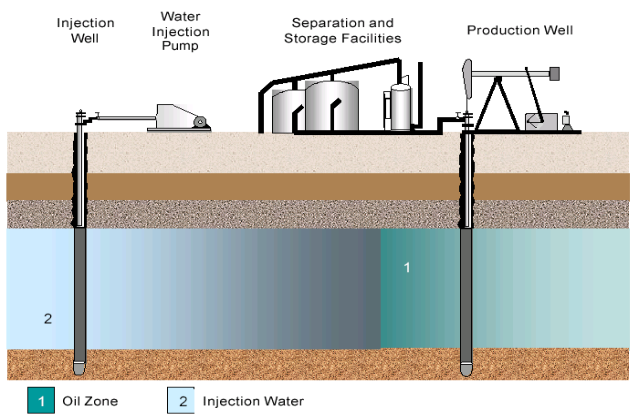
\includegraphics[scale=.7]{Fig/Waterflooding.PNG}
		\caption{Phương pháp bơm ép nước \cite{Petropedia}}
	\end{figure}
	\begin{figure}[h]
		\centering
		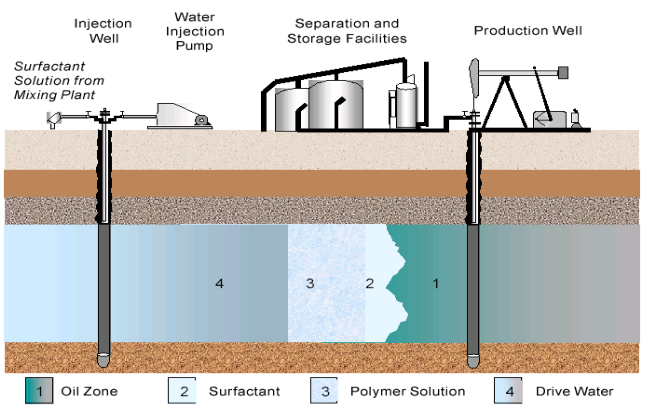
\includegraphics[scale=.7]{Fig/Chemical.PNG}
		\caption{Phương pháp bơm ép hóa chất \cite{el2017hydrophobic}}
	\end{figure}
	\clearpage
	\begin{figure}[h]
		\centering
		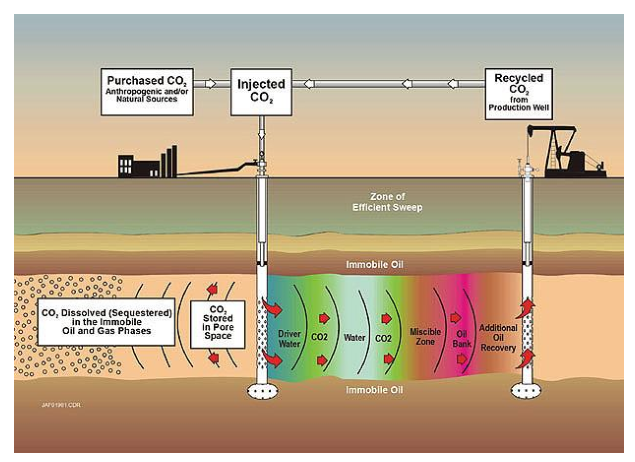
\includegraphics[scale=.7]{Fig/CO2.PNG}
		\caption{Bơm ép khí CO$_2$ \cite{CO2Solution}}
	\end{figure}
	\begin{figure}[h]
		\centering
		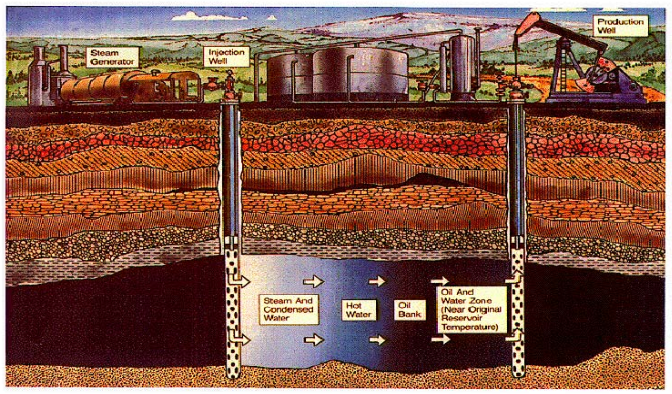
\includegraphics[scale=.55]{Fig/Thermal.PNG}
		\caption{Phương pháp nhiệt \cite{green1998enhanced}}
	\end{figure}
	\clearpage

\section{Cơ sở lý thuyết}
	\subsection{Thu hồi dầu tăng cường}
Thu hồi dầu tăng cường (Khai thác tam cấp hay EOR) là quá trình thu hồi dầu khí bằng cách bơm các tác nhân ngoại lai vào vỉa sản với mục đích khai thác tối đa các sản phẩm Hydrocacbon từ vỉa. Các phương pháp thu hồi dầu tăng cường bao gồm các nhóm chủ yếu sau: Nhóm phương pháp nhiệt, nhóm phương pháp hóa học, nhóm phương pháp khí trộn lẫn và phương pháp sử dụng nước đẩy (water flooding) có độ muối khoáng thấp \cite{green1998enhanced}. Mặc dù các (nhóm) phương pháp này yêu cầu những kĩ thuật cao, tốn kém và đôi khi không mang lại nhiều hiệu quả thu hồi nhưng các nhà nghiên cứu vẫn đặc biệt quan tâm đến tiềm năng thu hồi dầu tăng cường để có thể tăng sản lượng dầu khai thác trong nước.\\
Khai thác tam cấp được sử dụng khi những kĩ thuật khai thác sơ cấp hay thứ cấp không còn mang lại hiệu quả về kinh tế. Khai thác tam cấp đã được chứng minh là mang lại nhiều giá trị tại một số vùng của Hoa Kì bao gồm Utah, Texas và Mississipi, nơi những mỏ đã đi vào giai đoạn cuối của quá trình khai thác thứ cấp. Những mỏ này thường gây tổn thất nhiều chi phí nếu tiếp tục sử dụng những kĩ thuật khai thác thứ cấp, nhưng việc áp dụng khai thác tam cấp vẫn có thể mang về lợi nhuận đáng kể nếu giá dầu đủ cao.\\
Thu hồi dầu tăng cường bao gồm những phương pháp có kĩ thuật thu hồi phức tạp, liên quan đến việc bơm ép chất lỏng phi truyền thống vào vỉa để có thể nâng cao hệ số thu hồi dầu bằng cách giảm độ nhớt của lưu chất trong vỉa và tăng độ linh động của dầu. Khai thác tam cấp thường được áp dụng cho việc thu hồi dầu dư còn sót lại trong vỉa sau khi cả hai giai đoạn thu hồi sơ cấp và thứ cấp đã đạt tới giới hạn. Bao gồm những phương pháp nhiệt, hóa học, khí và sinh học được thể hiện trong Hình 5:
\clearpage
	\begin{figure}[h]
		\centering
		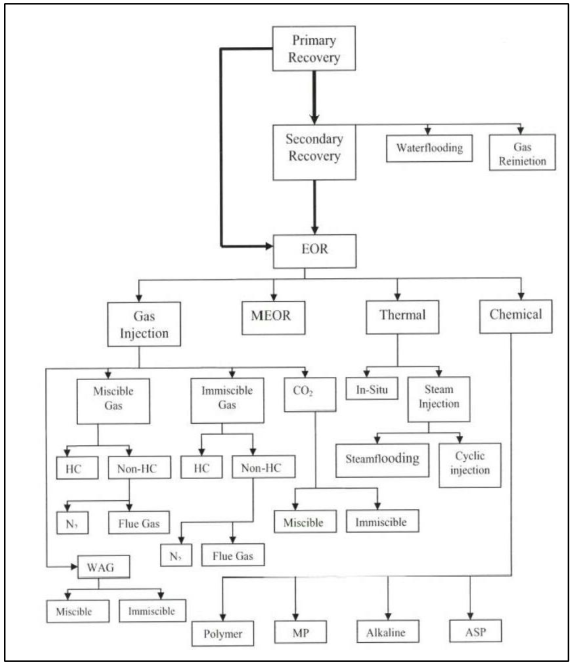
\includegraphics[scale=.7]{Fig/method.PNG}
		\caption{Những phương pháp khai thác dầu tăng cường \cite{doghaish2008analysis}}
	\end{figure}
%\newpage
	\subsection{Polymer flooding trong thu hồi dầu tăng cường}
	Polymer flooding nằm trong nhóm phương pháp hóa học, là phương pháp với hơn 40 năm phát triển và ứng dụng. Thể hiện được sự hiệu quả trong việc thu hồi dầu bằng cách thay đổi tỉ số độ nhớt. Thực tế cho thấy nhiều mỏ khi thực hiện polymer flooding có thể tăng lượng dầu thu hồi từ 5-30$\%$ \cite{abidin2012polymers} trữ lượng dầu ban đầu toàn mỏ (OIIP). Tổng chi phí cho phương pháp polymer flooding nhỏ hơn so với phương pháp water flooding do giảm bớt được hiện tượng khai thác nước trong khi khai thác dầu. Hiệu suất của phương pháp thường nằm trong khoảng 0.7-1.75lb polymer/bbl \cite{pope2007overview} dầu khai thác được.
	\subsubsection{Nguyên tắc và cơ chế}
	Polymer đóng vai trò quan trọng trong ngành công nghiệp dầu khí. Hầu hết những dự án sử dụng polymer flooding thường bao gồm pha trộn và bơm ép polymer vào giếng trong một khoảng thời gian nhất định cho đến khi 1/3-1/2 thể tích rỗng của vỉa được bơm ép \cite{abidin2012polymers}. Một thông số quan trọng được sử dụng cho phân tích cơ bản trước khi bơm polymer là tỉ số độ linh động. Tỉ số độ linh động biểu diễn mối quan hệ giữa độ thấm tương đối, độ nhớt của nước và độ nhớt của dầu trên một đơn vị tốc độ dòng chảy tỉ đối dựa trên định luật Darcy \cite{abidin2012polymers}:
		\begin{equation}
			f_o=\frac{1}{1+M}=\frac{1}{1+\mu_{o}k_w/\mu_{w}k_o}
		\end{equation}
	Dung dịch polymer đóng vai trò làm tăng độ nhớt và làm giảm độ thấm tương đối của dung dịch bơm ép khi được bơm vào vỉa. Do đó, làm giảm tỉ số độ linh động dẫn đến tốc độ dòng chảy tỉ đối của dầu tăng (theo phương trình (1)). Tốc độ dòng chảy tỉ đối của dầu cũng có thể được biểu diễn theo định luật Buckley-Leverett \cite{kantzas2012fundamentals}:
		\begin{equation}
			f_o=\frac{q_o}{q_w+q_o}
		\end{equation}
	Với: \hspace*{15pt} $q_o$ là lưu lượng dầu trong vỉa\\
	\hspace*{37pt} $q_w$ là lưu lượng nước trong vỉa.\\
	Khi tốc độ dòng chảy tỉ đối của dầu tăng, lưu lượng dầu trong vỉa cũng tăng. Kết quả đạt được là lượng dầu thu hồi tăng.\\
	Nếu tỉ số độ linh động bằng một hoặc gần bằng một, hiệu suất bơm ép polymer đạt mức tốt nhất. Ngược lại, nếu tỉ số độ linh động lớn hơn nhiều so với một, hiệu suất bơm ép là không đáng kể. Dựa vào nguyên lý thay đổi tỷ số độ nhớt, polymer có thể được sử dụng để tăng độ nhớt của pha nước trong khi làm giảm độ thấm tương đối của nước đối với không gian rỗng của đá trong vỉa và do đó tạo hiệu quả tốt nhất khi đẩy dầu ra khỏi vỉa. Mức độ hiệu quả của phương pháp tùy thuộc vào điều kiện vỉa với độ linh động của dầu bão hòa, thường lớn hơn không. Tuy nhiên, hiệu quả đáng kể thường thu được ở những vỉa có giá trị $k_o$ và độ linh động của dầu bão hòa tương đối cao.
	\newpage
	\subsubsection{Những polymer thông dụng}
	Hydrogel polymer được sử dụng thường xuyên trong EOR qua nhiều năm. Những hợp chất polymer này thường nằm dưới dạng chất lỏng phi Newton (còn gọi là chất lỏng giả dẻo). Polymer thường được sử dụng chung với các hợp chất hoạt động bề mặt (surfactants) hoặc phụ gia tính kiềm (alkaline) để có thể tăng hiệu suất quét của loại polymer được sử dụng. Trong khoảng 20 năm trở lại đây nhiều loại polymer mới được nghiên cứu, phát triển và đưa vào sử dụng. Những polymer mới đã thành công trong việc đáp ứng được nhiều điều kiện vỉa bao gồm:
	%\newpage
	\subsubsubsection{Hydrolyzed Polyacrylamides (HPAM)}
	Hydrolyzed polyacrylamide (HPAM) là một polymer tổng hợp trong nhóm polyacrylamide (PAM) có cấu tạo dạng mạch polymer thẳng của acrylamide đơn phân tử với một số phân tử bị thủy phân. Khối lượng phân tử có thể thay đổi linh động bằng cách thay đổi chuỗi cấu trúc phân tử của hợp chất. HPAM được sử dụng nhiều nhất trong các nhóm phương pháp polymer flooding do có khả năng thay đổi nhanh chóng độ nhớt dẻo và khả năng hòa tan trong nước tốt. Cấu trúc  được thể hiện trong Hình 6:
	\begin{figure}[h]
		\centering
		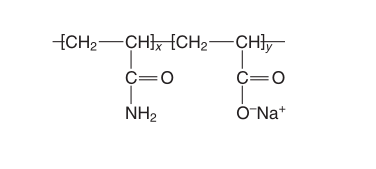
\includegraphics[scale=1]{Fig/HPAM.PNG}
		\caption{Cấu trúc phân tử HPAM \cite{sheng2010modern}}
	\end{figure}
	\newline
	Những loại HPAM được sử dụng trong EOR thường có khối lượng phân tử lớn hơn 20 triệu Daltons. Một số mỏ được ghi nhận sử dụng những loại HPAM cố khối lượng phân tử lớn hơn 35 triệu Daltons \cite{sheng2010modern}.\\
	Khối lượng phân tử của HPAM được thay đổi bằng cách thay đổi số lượng các nhóm carbonxyl và nhóm amide tùy thuộc vào nhu cầu sử dụng. Tuy nhiên nếu nhóm carboxyl chiếm hơn 40$\%$ thường dễ gây ra kết tủa nếu nước trong vỉa ở dạng nước cứng (nước chứa nhiều cation Ca$^{2+}$ và Mg$^{2+}$). Bởi vì quá trình EOR thường được thực hiện trong khoảng thời gian dài do đó nhóm amide thường chiếm mức độ lớn hơn. Đồng thời HPAM cũng không thích hợp cho những vỉa có nhiệt độ và độ khoáng hóa cao. 
	\subsubsubsection{Xanthan Gum/Biopolymer}
	Xanthan gum là một loại gôm hidrat cacbon cao phân tử do vi khuẩn lên men sinh ra và dùng trong quá trình tạo polime hay còn được gọi là polymer sinh học (biopolymer). Khối lượng phân tử của xanthan gum thường từ 1 triệu đến 15 triệu Daltons (trong EOR). Xanthan gum thường được sử dụng dưới hai dạng chính là dạng bột khô và dạng cô đặc \cite{sheng2010modern}. Cấu trúc của xanthan gum được thể hiện như Hình 7:
	\begin{figure}[h]
		\centering
		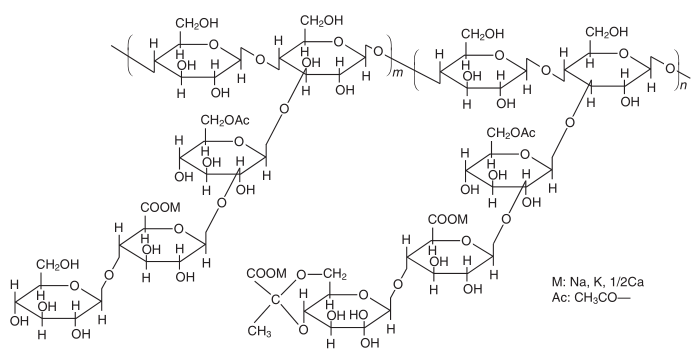
\includegraphics[scale=0.7]{Fig/xanthangum.PNG}
		\caption{Cấu trúc phân tử xanthan gum \cite{sheng2010modern}}
	\end{figure}
	\newline
	Tuy nhiên, polymer sinh học cũng dễ gây tắc nghẽn các kênh dẫn trong vỉa nếu sinh ra quá nhiều các đứt gãy tế bào. Bên cạnh đó, polymer sinh học dễ dàng bị phân hủy ở nhiệt độ trên 70$^o$C. Một số công ty có thể sử dụng những phương pháp kỹ thuật đặc biệt để có thể nâng khả năng chịu nhiệt tới 104$^o$C \cite{sheng2010modern}. Do được hình thành từ hoạt động của những vi sinh vật nên polymer sinh học cần được định kì thêm các chất phụ gia để ngăn chặn sự thoái hóa của vi sinh vật.
	\newpage
	\subsubsubsection{Salinity-Tolerant Polyacrylamide (KYAPM)}
	Được biết đến là một loại polymer có khả năng chịu mặn, thích hợp sử dụng ở những vỉa có độ muối khoáng cao. Cấu trúc của KYPAM được thể hiện như Hình 8:
	\begin{figure}[h]
		\centering
		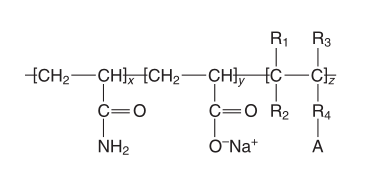
\includegraphics[scale=1]{Fig/KYPAM.PNG}
		\caption{Cấu trúc phân tử KYPAM \cite{sheng2010modern}}
	\end{figure}
	\newline
	Với $R_1, R_2$ và $R_3$ là những gốc alkyl từ $C_1 - C_{12}$. A là những nhóm ion có khả năng hạn chế các cation Ca$^{2+}$ và Mg$^{2+}$. $R_1, R_2$ và $R_3$ ảnh hưởng trực tiếp đến độ dẻo của polymer, nếu tăng số lượng phân tử carbon trong ba nhóm này sẽ làm tăng tính dẻo của polymer. Nhóm $R_4$ ảnh hưởng đến độ chịu mặn của polymer, tăng số lượng phân tử carbon sẽ làm tăng khả năng chịu mặn của polymer \cite{sheng2010modern}. 
	\noindent
	Bảng 1 thể hiện các tính chất hóa lý của polymer theo tiêu chuẩn Q/DQ0977-1996 của Daqing Industry Specification.
\begin{table}[h]
\centering
\caption{So sánh tính chất lý hóa của KYPAM và HPAM \cite{sheng2010modern}}
\label{my-label}
\begin{tabularx}{\textwidth}{@{}XXX@{}}
\toprule
\textbf{Thông số} & \textbf{KYPAM} & \textbf{HPAM} \\ \midrule
Trạng thái                         & Bột trắng                       & Bột trắng                      \\
Hàm lượng rắn (\%)                 & 90                              & 90.2                           \\
Khối lượng phân tử (Triệu)       & 25.14                           & 17                             \\
Độ thủy hóa (\% mol)               & 26.4                            & 26.8                           \\
Thời gian hòa tan (h)              & $\leq$2                         & $\leq$2                        \\
Thành phần không tan (\%)     & 0.115                           & 0.19                           \\
Lượng dư phân tử (\%)             & 0.0096                          & 0.021                          \\
Chỉ số thấm lọc                   & 1.12                            & 1.22                           \\
Hệ số khuếch tán                 & 102.6                           & 41.3                           \\ \bottomrule
\end{tabularx}
\end{table}
	\newpage
	\subsubsubsection{2-Acrylamide-2-Methyl Propane-Sulfonate Copolymer}
	Cấu trúc của AMPS/AM được thể hiện như Hình 9:\\
	\begin{figure}[h]
		\centering
		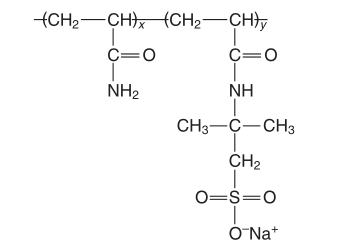
\includegraphics[scale=0.7]{Fig/AMPS.PNG}
		\caption{Cấu trúc phân tử AMPS \cite{sheng2010modern}}
	\end{figure}
	\newline
	Là một loại polymer đồng trùng hợp giữa các gốc Natri và Sulfonate, acrylamide và một số chất hòa tan trong nước. Do có gốc sulfonate, loại polymer này mang lại nhiều ưu điểm như khả năng trao đổi ion, tính dẫn điện, mức độ chịu mặn tốt. Nhóm acrylamide mang lại khả năng bền nhiệt cao, độ kháng thủy hóa, acid, alkaline cao. AMPS/AM có khả năng chịu nhiệt, chịu mặn tốt hơn gấp hai lần so với HPAM ở cùng một điều kiện \cite{sheng2010modern}. Tuy nhiên, những tính chất đặc biệt này làm cho giá thành của polymer đồng trùng hợp thường rất cao.
	\subsubsubsection{New polymer}
	Polymer đang ngày một trở nên quan trọng trong công nghiệp dầu khí. Do tính chất của quá trình khai thác dầu khí, vì vậy những polymer đang được áp dụng như xanthan, HPAM không còn thích hợp trong điều kiện vỉa khắc nhiệt. Yêu cầu cấp thiết cần tạo ra loại những loại polymer mới đáp ứng được những yêu cầu khai thác trong tương lai. 	
		\begin{enumerate}
			\item Polymer tổng hợp
		\end{enumerate}
	Polymer tổng hợp được coi là một giải pháp tuyệt vời kết hợp giữa polymer sinh học và polymer chịu nhiệt, muối khoáng cao \cite{sorbie2013polymer}. Polymer tổng hợp vẫn giữ nguyên được những tính chất cơ bản của polymer như khối lượng phân tử lớn để có thể dễ dàng kiểm soát tỉ số độ linh động dựa trên mối quan hệ giữa nồng độ và độ nhớt. Đồng thời dựa trên nhiều thí nghiệm đã chứng tỏ được tính chất bền với nhiệt và nâng cao độ bền cắt \cite{sorbie2013polymer}. Nhiều polymer tổng hợp chứng tỏ được nhiều lợi thế hơn so với xanthan hay HPAM, tiêu biểu là polymer acrylamide đồng trùng hợp (Acrylamide co-polymer). Tuy nhiên, polymer tổng hợp vẫn còn đang trên giai đoạn nghiên cứu và chưa đưa ra được hiệu quả thực tế nào, đồng thời cấu trúc của polymer tổng hợp vẫn còn là một vấn đề làm đau đầu nhiều nhà khoa học. 
		\begin{enumerate}
			\item[2.] Polymer sinh học cải tiến (Improved biopolymer)
		\end{enumerate}
	Dựa trên sự nghiên cứu về những thay đổi về tính chất của xanthan trong các môi trường khác nhau để có thể thay đổi nhằm cải thiện tính chất của xanthan. Dựa trên sự phát triển của vi sinh vật và nấm để có thể thay đổi các tính chất như độ nhớt, độ ổn định, tăng cường khả năng chịu nhiệt. Hình dạng và cấu trúc của loại polymer này làm cho nó có độ nhớt cao với mức độ ổn định lớn, cực kỳ thích hợp để ứng dụng trong thu hồi dầu tăng cường \cite{sorbie2013polymer}. Loại polymer này đang đem lại rất nhiều hy vọng cho ngành công nghiệp khai thác dầu khí trong tương lai. Tuy nhiên, thông qua nhiều thí nghiệm cho thấy khả năng bơm ép của polymer sinh học cải tiến khá thấp do tính chất dễ bị kết tụ thành khối khi tiến hành bơm ép, điều này làm cho việc thực hiện tiêu tốn nhiều kinh phí và không phù hợp với thời điểm hiện tại.
	\newpage
	\subsubsection{Những tính chất cơ bản}
	\subsubsubsection{Độ nhớt}
	Khi nồng độ polymer đủ cao, polymer hầu như luôn thể hiện tính chất của lưu chất phi Newton. Nồng độ polymer càng cao, độ nhớt của polymer càng lớn (Hình 10).
		\begin{figure}[h]
			\centering
			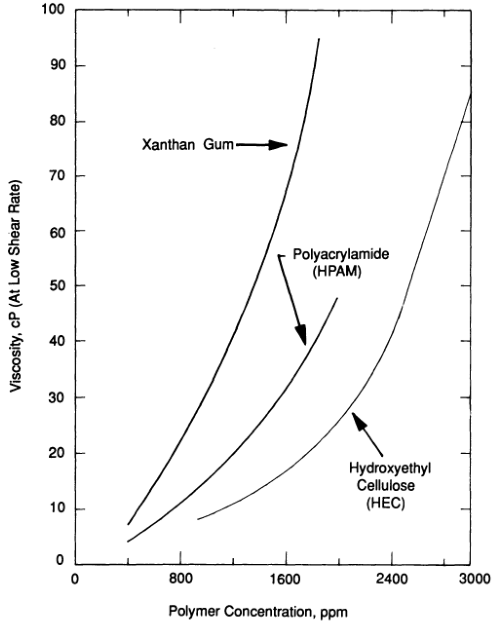
\includegraphics[scale=.8]{Fig/concentration.PNG}
			\caption{Tương quan nồng độ-độ nhớt (shear rate: $7.3s^-1$, 1\% NaCl tại 74$^\circ$F) \cite{sorbie2013polymer}}
		\end{figure}
	\subsubsubsection{Tính chất lưu biến}
		\begin{figure}[h]
			\centering
			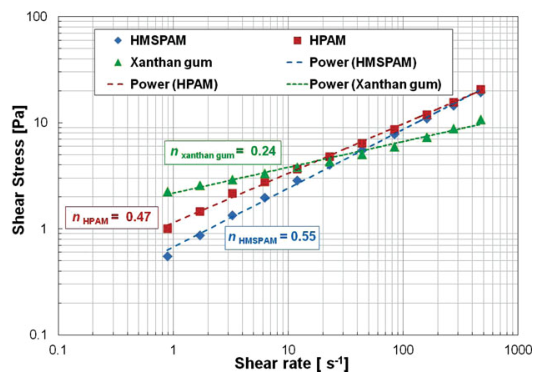
\includegraphics[scale=.9]{Fig/Shearstress.PNG}
			\caption{Ứng suất cắt của HPAM, HMSPAM và xanthan \cite{wei2014mechanical}}
		\end{figure}
	\newline
	Hình 11 thể hiện ứng suất cắt của ba loại polymer HPAM, HMSPAM và xanthan thông qua tốc độ trượt. Ứng xử của dòng chảy được thể hiện bằng mô hình hàm mũ với HPAM, HMSPAM lần lượt là 0.47 và 0.55, trong khi xanthan là 0.24 (độ cắt mỏng lớn (stronger shear-thinning)). Những phân tử xanthan được liên kết thông qua liên kết hidro (hydrogen bonding) và liên kết bẫy phân tử, vì vậy, xanthan thường có độ nhớt cao ở tốc độ trượt thấp. Ở tốc độ trượt cao, các liên kết bẫy phân tử cao dễ bọ phá vỡ làm giảm độ nhớt của của xanthan. Tính chất này cũng đúng với HPAM và hầu hết các loại polymer ứng dụng trong công nghiệp dầu khí khác.
	\subsubsubsection{Độ ổn định}	
	Khi polymer được sử dụng để bơm ép vào trong vỉa, polymer sẽ bắt đầu bị thoái biến, độ ổn định của polymer là một tính chất cực kỳ quan trọng để giữ cho polymer giảm thiểu tối đa mức độ thoái biến. Thoái biến là quá trình phá vỡ các cấu trúc phân tử polymer \cite{sorbie2013polymer}, có thể do các nguyên nhân sau:
		\begin{itemize}
			\item Thoái biến do nguyên nhân hóa học: bị thoái biến do hoạt động của các chất khác như oxy hay quá trình thủy phân.
			\item Thoái biến do nguyên nhân cơ học: bị phá vỡ cấu trúc phân tử khi đi vào những vùng có xuất hiện dòng lưu lượng cao, nhiệt độ cao.
			\item Thoái biến do nguyên nhân sinh học: chủ yếu do sự hoạt động của vi sinh vật.
		\end{itemize}
	Tăng độ ổn định cho polymer:
		\begin{enumerate}
			\item Tăng độ ổn định hóa học:
			\begin{itemize}
				\item Lựa chọn nhiều loại polymer
				\item Thêm chất phụ gia chống oxy hóa và thủy phân
				\item Kiểm tra giới hạn chịu đựng (muối, pH...) trong điều kiện vỉa.
			\end{itemize}
			\item Tăng độ ổn định cơ học:
			\begin{itemize}
				\item Tăng khối lượng phân tử
				\item Tăng độ nhớt, độ bền gel
				\item Tăng kích thước phân tử
				\item Tăng giới hạn ứng suất cắt.
			\end{itemize}
			\item Tăng độ ổn định sinh học:
			\begin{itemize}
				\item Thêm phụ gia chống sự hoạt động của vi sinh vật.
			\end{itemize}
		\end{enumerate}

	\subsubsection{Hiệu suất đẩy}
	Hiệu suất đẩy thường quyết định quá trình thu hồi dầu tăng cường thành công hay thất bại. Hiệu suất đẩy được nghiên cứu dựa trên những nghiên cứu về độ bão hòa dầu dư, nhưng hiện tại chưa có một tiêu chuẩn thống nhất nào cho chỉ số này. Phương trình (3) thể mối quan hệ giữa hiệu suât đẩy và độ bão hòa dầu trong vỉa \cite{green1998enhanced}.
		\begin{equation}
			E_D=(S_{oi}-S_{or})/S_{oi}
		\end{equation}
	Có nhiều yếu tố ảnh hưởng đến hiệu suất quét như cấu trúc phân tử của polymer hay độ nhớt dẻo. Bơm ép polymer thường mang lại hiệu suất quét cao do polymer có độ nhớt dẻo lớn làm thay đổi tính chất dòng chảy trong vỉa (tuân theo định luật Reynolds). 

	\subsubsection{Hiệu suất quét}
	Mang lại hiệu suất quét ($E_A$) cao chính là chìa khóa quan trọng nhất làm nên thành công của phương pháp bơm ép polymer \cite{sheng2010modern}. Có thể tăng hiệu suất quét bằng nhiều cách như thay đổi vị trí đặt giếng, bơm ép theo từng phân lớp, thay đổi và kiểm soát tính chất polymer bơm ép.\\
	Độ nhớt của polymer là yếu tố chính để có thể nâng cao hiệu suất quét của polymer. Trong một số tư liệu chỉ ra rằng độ nhớt của pha chất lưu thay thế nên được kiểm soát ở mức độ bằng với độ nhớt của pha chất lưu bị thay thế. Tuy nhiên, trong thực tế độ nhớt của polymer thường cao gấp 3 đến 5 lần độ nhớt của dầu, mục đích là để đạt được hiệu suất cao nhất có thể trong môi trường vỉa bất đồng nhất.\\

	\subsection{Tỉ số độ linh động}
	\subsubsection{Định nghĩa}
	Độ linh động của một chất lưu (i) được định nghĩa như sau \cite{kantzas2012fundamentals}:
		\begin{equation}
			\lambda_i = \frac{k_i}{\mu_i}
		\end{equation}
	Với:\hspace{15pt} $\mu_i$ là độ nhớt của chất lưu\\
		 \hspace*{37pt}$k_i$ là độ thấm hiệu dụng của đá đối với chất lưu i.\\
	Tỉ số độ linh động (M) \cite{kantzas2012fundamentals} là tỉ số của pha chất lưu thay thế đối với pha chất lưu bị thay thế. Tỉ số độ linh động là một trong những thông số quan trọng nhất trong quá trình bơm ép polymer, ảnh hưởng trực tiếp đến hiệu suất quét của polymer.
		\begin{equation*}
			M = \frac{\lambda_D}{\lambda_d} = \frac{\mu_d}{\mu_D}
		\end{equation*}
	Với: \hspace{15pt}$\lambda_D$ là độ linh động của pha chất lưu thay thế\\
	\hspace*{37pt}$\lambda_d$ là độ linh động của pha chất lưu bị thay thế\\
	\hspace*{37pt}$\mu_D$ là độ nhớt của pha chất lưu thay thế\\
	\hspace*{37pt}$\mu_d$ là độ nhớt của pha chất lưu bị thay thế.\\
	Khi giá trị M nhỏ hơn 1 được gọi là tỉ số độ linh động thích hợp (favorable) thuận lợi để triển khai phương pháp EOR, ngược lại khi giá trị của M lớn hơn 1 được gọi là tỉ số độ linh động không thích hợp (unfavorable). Biểu đồ Hình 12 thể hiện mối tương quan giữa tỉ số độ linh động và hiệu suất quét $E_A$. Khi M bắt đầu tăng hiệu suất quét sẽ giảm, đặc biệt là khi M vượt qua giá trị 1, $E_A$ bắt đầu giảm mạnh. Hiệu suất đẩy khi tỉ số độ linh động cao thường thấp chủ yếu là do M quá lớn dẫn đến hiện tượng tạo ngón và phá vỡ phân bố hình học khi bơm ép. 
		\begin{figure}[h]
			\centering
			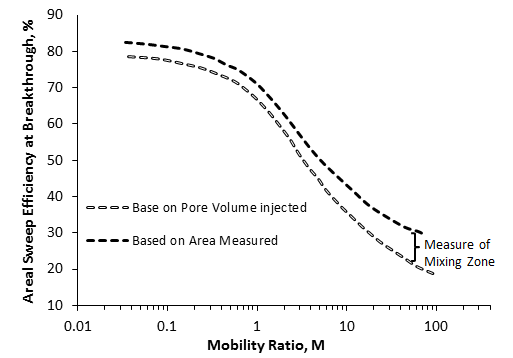
\includegraphics[scale=1]{Fig/M.PNG}
			\caption{Mức độ tương quan giữa hệ số quét và tỉ số độ linh động \cite{kantzas2012fundamentals}}
		\end{figure}
	\newline
	Khi sử dụng phương pháp bơm ép nước dễ xảy ra những hiện tượng trên do tỉ số độ linh động không thích hợp, khi đó dung dịch polymer sẽ được đưa vào sử dụng nhằm làm giảm tỉ số độ linh động. Tuy nhiên, trong những đơn giản chỉ cần giảm tỉ số độ linh động gần băng một, ở những vỉa có mức độ bất đồng nhất cao việc làm sao để có thể giảm tỉ số độ linh động xuống dưới một là điều rất quan trọng, điều này quyết định tới hệ số quét và hệ số đẩy khi sử dụng bơm ép polymer. 

	\subsubsection{Yếu tố ảnh hưởng}
	\textbf{Nồng độ polymer:} Mục đích chính của việc thêm polymer vào trong dung dịch bơm ép là để gia tăng độ nhớt của dung dịch. Độ nhớt dung dịch bơm ép cao thường mang lại hiệu quả lớn trong việc tăng hiệu suất quét, ngăn chặn quá trình đẩy nước và tạo kênh dẫn. Ảnh hưởng của nồng động polymer lên độ nhớt dung dịch được thể hiện trong Bảng 2. Hoàn toàn dễ thấy rằng khi tăng nồng độ polymer sẽ làm tăng độ nhớt dung dịch.
	
	\begin{table}[h]
	\centering
	\caption{Ảnh hưởng của nồng độ polymer lên độ nhớt \cite{nguyen2015effective}}
	\label{my-label}
	\begin{tabular}{@{}lcc@{}}
	\toprule
	\textit{STT} & \multicolumn{1}{l}{\textit{Nồng độ polymer, wt\%}} & \multicolumn{1}{l}{\textit{Độ nhớt dung dịch, cp (for NaOH)}} \\ \midrule
	1 & 0.1 & 3.31 \\
	2 & 0.3 & 4.32 \\
	3 & 0.5 & 5.85 \\
	4 & 0.8 & 9.93 \\
	5 & 1 & 12.93 \\ \bottomrule
	\end{tabular}
	\end{table}

	\noindent
	\textbf{Nhiệt độ:} Khi tăng nhiệt độ lưu chất, các phần tử hạt trong lưu chất di chuyển nhanh hơn, có xu hướng tách rồi khỏi những phần tử xung quanh. Do đó, khi nhiệt độ tăng độ nhớt của dung dịch sẽ giảm đáng kể.\\
	\textbf{Lực hút:} Những phần tử hạt nhỏ trong cùng một loại hợp chất thường tác động một lực hút lên các phần tử xung quanh. Lực hút này cũng đồng thời ảnh hưởng đến độ nhớt, lực hút càng lớn độ nhớt dung dịch càng cao.\\
	\textbf{Kích thước hạt:} Kích thước hạt có ảnh hưởng đáng kể đến độ nhớt của dung dịch. Kích thước hạt nhỏ làm cho các phần tử hạt dễ di chuyển hơn, tốc độ dòng chảy nhanh hơn đồng nghĩa với độ nhớt thấp hơn.
	\subsection{Độ thấm tương đối}
	Độ thấm tương đối của một chất lưu là một đại lượng đo đạt không thứ nguyên của độ thấm hiệu dụng đối với pha chất lưu đó. Độ thấm tương đối là tỉ số giữa độ thấm hiệu dụng của một pha chất lưu đối với độ thấm tuyệt đối của pha chất lưu đó.\\
	Độ thấm tương đối phụ thuộc vào hình dạng lỗ rỗng, độ ẩm, phân bố chất lưu và quá trình bão hòa chất lưu. Các phép đo độ thấm tương đối được tiến hành trên các mẫu lõi trong phòng thí nghiệm, thường tốn nhiều thời gian và chi phí do đó thường chỉ được thực hiện trong gia đoạn khai thác thứ cấp hoặc tam cấp.\\
	Trong hệ hai pha, các chất lưu có thể là dầu - nước hoặc dầu - khí. Trong hệ ba pha, cả ba loại lưu chất sẽ cùng tồn tại. Mỗi lưu chất khi chảy trong mỗi trường rỗng luôn bị tác động bởi lực mao dẫn tồn tại bên trong các kênh dẫn, làm giảm tốc độ dòng chảy của từng pha riêng lẻ theo một hàm phi tuyến. Do đó, tổng độ thấm tương đối của mỗi pha luôn nhỏ hơn một.
	\subsection{Mô hình sandpack}
	\subsubsection{Mô hình sandpack một chiều}
	Hệ thống thí nghiệm sandpack một chiều bao gồm một ống kính có chiều dài 1-ft, đường kính trong 1-in được chứa đầy cát (sandpack column). Sandpack column phải được làm khô, trừ những trường hợp thí nghiệm đặc biệt \cite{li2011study}. Cát liên tục được nén chặt cho đến khi đầy ống thủy tinh. Hai đầu được bịt kín bằng các nút cao su, một màng kim loại được đặt giữa nút cao su và cát.\\
	Độ rỗng của mô hình được đo bằng phương pháp sau. Sandpack column được bơm khí CO$_2$ dưới áp suất nhẹ (khoảng 2.5 psig) trong vòng 30 phút để có thể đẩy được hết không khí còn chứa trong lỗ rỗng, sau đó sandpack column tiếp tục được bơm ép một được nước tinh khiết cho đến khi hòa tan hết lượng khí CO$_2$ và chiếm toàn bộ phần thể tích rỗng trong cột. Thể tích rỗng sẽ tương đương tổng thể tích nước được bơm vào trong sandpack. Thể tích tổng của cả sandpack chính là tích của chiều dài và diện tích mặt cắt của sandpack. Như vậy, độ rỗng của sandpack được tính như sau \cite{li2011study}:
		\begin{equation}
			\phi=\frac{V_{H_2O}}{\frac{\pi.D
			^2.L}{4}}
		\end{equation}
	Với $D$ là đường kính trong của Sandpack, $L$ là chiều dài của sandpack. Độ rỗng đo được thường thấp hơn so với giá trị trong lý thuyết do mức độ phân bố kích thước hạt trong sanpack.\\Độ thấm $k$ có thể được tính theo định luật Darcy cho chất lỏng đơn pha \cite{li2011study}:
		\begin{equation}
			\bar u =-\frac{k}{\mu}(\triangledown p-\rho \bar g)
		\end{equation}
	Với $u, \mu, \rho$ lần lượt là vận tốc, độ nhớt và tỉ trọng chất bơm ép. Trong những thí nghiệm sandpack nằm ngang có thể bỏ qua ảnh hưởng của lực trọng trường \cite{li2011study}:
		\begin{equation}
			u=\frac{k}{\mu}.\frac{\Delta p}{L}
		\end{equation}
	Với $\Delta p$ là chênh áp, $L$ là khoảng cách giữa hai đầu.
		\begin{figure}[h]
			\centering
			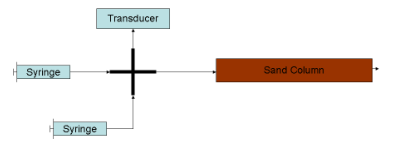
\includegraphics[scale=1]{Fig/1d-sanpack.PNG}
			\caption{Sơ đồ bố trí mô hình thí nghiệm sanpack một chiều \cite{li2011study}}
		\end{figure}
	\newpage
	\subsubsection{Mô hình sandpack hai chiều}
	\subsubsubsection{Cấu trúc}
	Mô hình sandpack hai chiều hay còn gọi là mô hình sandpack không đồng nhất. Được thiết kế từ thép không rỉ gắn với một lớp kính có độ dày 1.25-in phía trước để có thể dễ dàng quan sát. Bên trong là một ngăn nhỏ có kích thước 20x3x0.75-in như Hình 14.
		\begin{figure}[h]
			\centering
			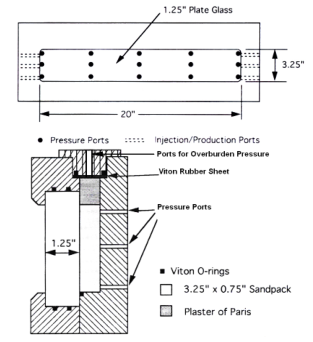
\includegraphics[scale=1]{Fig/2dsandpack1.PNG}
			\caption{Mô hình sandpack 2-D nhìn từ trước và mặt bên \cite{li2011study}}
		\end{figure}
		\begin{figure}[h]
			\centering
			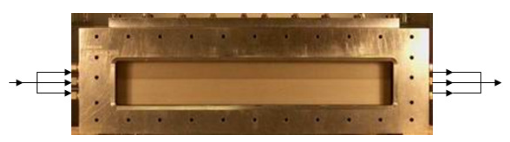
\includegraphics[scale=1]{Fig/2dsandpack2.PNG}
			\caption{Mô hình sandpack 2-D (mũi tên chỉ hướng dòng lưu chất được bơm ép) \cite{li2011study}}
		\end{figure}
	\newline
	Mô hình sử dụng cát silic oxit làm phân làm 2 lớp với độ thấm khác nhau. Một lớp sử dụng cát hạt thô với độ thấm cao (phía trên), lớp còn lại sử dụng cát hạt mịn với độ thấm thấp (phía dưới). Tỉ lệ độ dày giày giữa hai lớp là 2:3, tỉ lệ độ thấm là 19:1, tương ứng 90 và 4.8 Darcy, độ thấm của mỗi lớp được đo bằng mô hình sandpack 1-D. Tổng thể tích rỗng của mô hình (TPV) là 330 mL, độ rỗng tổng là 0.38 và độ thấm tổng đo được là 39 Darcy. Độ thấm được đo bằng cách bơm ép lưu chất vào mô hình và sử dụng định luật Darcy để tính toán. Trong thí nghiệm, quá trình waterflood sử dụng nước biển với nồng độ NaCl là 3.0 \%wt, độ nhớt là 1.15 mPa.s ở 22.5$^{\circ}$C. Polymer được sử dụng trong thí nghiệm thuộc loại HPAM, có tên AN 930 PGO, được cung cấp bởi SNF Floerger (Pháp). Độ thủy phân và khối lượng phân tử tương đối của AN 930 PGO tương ứng là 25 \%mol và $18\times10^6$, độ nhớt được đo bằng nhớt kế Brookfeild DV-II+ tại nhiệt độ phòng.
	\subsubsubsection{Độ thấm tổng}
	Khi dòng lưu chất (thường là nước) chảy qua một thớ gồm $n$ lớp song song, độ thấm tổng của $n$ lớp được xem như là trung bình của các lớp với độ thấm $k_i$ và độ dày $h_i$ \cite{li2011study}.
		\begin{equation}
			k_{overall}=\sum_{i=1}^nk_ih_i/\sum_{i=1}^nh_i
		\end{equation}
	Tỉ lệ độ dày giữa hai lớp là 2:3, như vậy độ thấm tổng sẽ là:
		\begin{equation}
			k_{overall}=\frac{90\times0.4h+4.8\times0.6h}{0.4h+0.6h}\approx39 Darcy
		\end{equation}

\newpage
\section{Case Study}
	Thí nghiệm được thực hiện bởi Wassmuth, F.R., Green, K., Hodgins, L., Turta, năm 2007 \cite{wassmuth2007polymer} với đối tượng là các mẫu dầu có độ nhớt lần lượt là 430 mPa.s, 1108 mPa.s, 1450 mPa.s, 2900 mPa.s và 5500 mPa.s. Các mẫu dầu lần lượt được thực hiện thí nghiệm trong mô hình sandpack-column cùng với 29 mẫu polymer có độ nhớt khác nhau để chỉ ra mối quan hệ giữa lượng dầu thu hồi tăng cường với độ nhớt của polymer và độ nhớt của dầu. Mọi quá trình bơm ép polymer đều được thực hiện sau quá trình bơm ép nước. Mọi dữ liệu thu được sau thí nghiệm được thể hiện trong phụ lục A \cite{wang2009optimum}.
	\subsection{Độ thấm tương đối dầu-nước}
	Mức độ tương quan giữa độ thấm tương đối của dầu-nước được thể hiện thông qua đường cong Corey, trong đó:\\
	Độ thấm tương đối của dầu \cite{guliyev2008simulation}:
		\begin{equation}
			k_{ro}=(1-S_{wD})^{n_o}
		\end{equation}
	Độ thấm tương đối của nước \cite{guliyev2008simulation}:
		\begin{equation}
			k_{rw}=S_{wD}^{n_w}
		\end{equation}
	Với:\hspace*{15pt}$S_{wD}$ là độ bão hòa của nước trong hệ có hai độ rỗng khác nhau, được tính theo công thức (12) \cite{guliyev2008simulation}:
		\begin{equation}
			S_{wD}=\frac{S_w-S_{wi}}{1-S_{wi}-S_{or}}
		\end{equation}
	Với $n_o=2$, $n_w=1.8$ lần lượt là các giá trị hệ số mũ của dầu và nước được lựa chọn dựa trên pha không dính ướt trong thí nghiệm.\\
	Sau khi chuẩn bị và thực hiện đầy đủ các bước đầu của thí nghiệm, tiếp theo đầu thô sẽ được bơm ép vào trong sandpack-column cho đến khi không còn nước chảy ra từ trong sandpack-column nữa - lượng dầu này được xem là lượng dầu ban đầu trong sandpack (OOIP, $cm^3$). Độ bão hòa nước ban đầu ($S_{wi}$) được tính toán dựa trên OOIP và thể tích nước bơm ép (PV, $cm^3$) sau khi thực hiện waterflood như sau \cite{pereira2014ionic}:
		\begin{equation}
			S_{wi}=\frac{PV-OOIP}{PV}\times{100}
		\end{equation}
	\newpage
	\noindent
	Sau khi thực hiện waterflood, thể tích lượng dầu thu hồi ($S_{orwf}, cm^3$) được xác định. Độ bão hòa dầu dư ($S_{or}$) được tính theo công thức sau \cite{pereira2014ionic}:
		\begin{equation}
		S_{or}=\frac{OOIP-S_{orwf}}{OOIP}\times{100}
		\end{equation}
	Mức độ tương quan giữa độ thấm tương đối dầu-nước được thể hiện qua đường cong Corey.
		\begin{figure}[h]
			\centering
			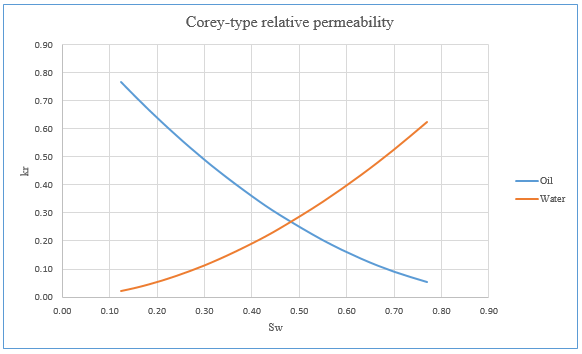
\includegraphics[scale=1]{Fig/Corey.PNG}
			\caption{Tương quan Corey cho độ thấm tương đối}
		\end{figure}
	\newline
	Các giá trị độ thấm tương đối, độ bão hòa được tính toán như trong Bảng 3, Bảng 4, Bảng 5, Bảng 6 và Bảng 7 tương ứng với các mẫu dầu có độ nhớt 430 mPa.s, 1108 mPa.s, 1450 mPa.s, 2900 mPa.s và 5500 mPa.s.
\begin{table}[h]
\centering
\caption{Dầu có độ nhớt 430 mPa.s}
\label{my-label}
\begin{tabularx}{\textwidth}{@{}XXXXXXXXXX@{}}
\toprule
No. & $S_w$ & $S_{wD}$ & $S_{orwf}$ & $S_{or}$ & $S_{wi}$ & $k_{ro}$ & $k_{rw}$ \\ \midrule
1   & 0.15  & 0.12     & 1.3        & 0.581    & 0.112    & 0.77     & 0.02     \\
2   & 0.17  & 0.19     & 1.51       & 0.576    & 0.109    & 0.65     & 0.05     \\
3   & 0.24  & 0.39     & 1.17       & 0.582    & 0.125    & 0.37     & 0.19     \\
4   & 0.31  & 0.66     & 0.98       & 0.598    & 0.133    & 0.12     & 0.47     \\
5   & 0.35  & 0.81     & 0.93       & 0.598    & 0.135    & 0.04     & 0.68     \\ \bottomrule
\end{tabularx}
\end{table}
\begin{table}[h]
\centering
\caption{Dầu có độ nhớt 1108 mPa.s}
\label{my-label}
\begin{tabularx}{\textwidth}{@{}XXXXXXXXXX@{}}
\toprule
No. & $S_w$ & $S_{wD}$ & $S_{orwf}$ & $S_{or}$ & $S_{wi}$ & $k_{ro}$ & $k_{rw}$ \\ \midrule
1   & 0.2   & 0.35     & 1.65       & 0.597    & 0.092    & 0.43     & 0.15     \\
2   & 0.21  & 0.33     & 2          & 0.578    & 0.106    & 0.45     & 0.14     \\
3   & 0.24  & 0.37     & 1.82       & 0.581    & 0.133    & 0.39     & 0.17     \\
4   & 0.26  & 0.48     & 1.94       & 0.58     & 0.112    & 0.27     & 0.27     \\
5   & 0.28  & 0.55     & 1.9        & 0.582    & 0.11     & 0.20     & 0.34     \\
6   & 0.31  & 0.66     & 1.78       & 0.585    & 0.108    & 0.12     & 0.47     \\
7   & 0.35  & 0.78     & 1.95       & 0.58     & 0.105    & 0.05     & 0.64     \\ \bottomrule
\end{tabularx}
\end{table}

\begin{table}[h]
\centering
\caption{Dầu có độ nhớt 1450 mPa.s}
\label{my-label}
\begin{tabularx}{\textwidth}{@{}XXXXXXXXXX@{}}
\toprule
No. & $S_w$ & $S_{wD}$ & $S_{orwf}$ & $S_{or}$ & $S_{wi}$ & $k_{ro}$ & $k_{rw}$ \\ \midrule
1  & 0.15  & 0.13     & 3.66       & 0.573    & 0.107    & 0.75     & 0.03     \\
2  & 0.17  & 0.19     & 4.05       & 0.578    & 0.111    & 0.66     & 0.05     \\
3  & 0.24  & 0.45     & 3.92       & 0.575    & 0.086    & 0.30     & 0.24     \\
4  & 0.29  & 0.59     & 3.03       & 0.578    & 0.101    & 0.17     & 0.39     \\
5  & 0.34  & 0.75     & 3.28       & 0.581    & 0.109    & 0.06     & 0.59     \\ \bottomrule
\end{tabularx}
\end{table}

\begin{table}[h]
\centering
\caption{Dầu có độ nhớt 2900 mPa.s}
\label{my-label}
\begin{tabularx}{\textwidth}{@{}XXXXXXXXXX@{}}
\toprule
No. & $S_w$ & $S_{wD}$ & $S_{orwf}$ & $S_{or}$ & $S_{wi}$ & $k_{ro}$ & $k_{rw}$ \\ \midrule
1   & 0.17  & 0.2      & 3.86       & 0.591    & 0.11     & 0.64     & 0.06     \\
2   & 0.19  & 0.26     & 4.78       & 0.59     & 0.111    & 0.54     & 0.09     \\
3   & 0.23  & 0.39     & 5.05       & 0.596    & 0.119    & 0.37     & 0.18     \\
4   & 0.26  & 0.47     & 4.84       & 0.576    & 0.115    & 0.29     & 0.26     \\
5   & 0.33  & 0.71     & 4.28       & 0.585    & 0.125    & 0.09     & 0.54     \\ \bottomrule
\end{tabularx}
\end{table}

\begin{table}[h]
\centering
\caption{Dầu có độ nhớt 5500 mPa.s}
\label{my-label}
\begin{tabularx}{\textwidth}{@{}XXXXXXXXX@{}}
\toprule
No. & $S_w$ & $S_{wD}$ & $S_{or}$ & $S_{wi}$ & $k_{ro}$ & $k_{rw}$ \\ \midrule
1   & 0.14  & 0.11     & 0.59     & 0.107    & 0.79     & 0.02     \\
2   & 0.16  & 0.18     & 0.584    & 0.105    & 0.68     & 0.04     \\
3   & 0.22  & 0.38     & 0.586    & 0.102    & 0.39     & 0.17     \\
4   & 0.25  & 0.44     & 0.577    & 0.115    & 0.32     & 0.23     \\
5   & 0.28  & 0.55     & 0.574    & 0.105    & 0.21     & 0.34     \\
6   & 0.33  & 0.73     & 0.589    & 0.111    & 0.07     & 0.57     \\
7   & 0.36  & 0.81     & 0.579    & 0.107    & 0.04     & 0.68     \\ \bottomrule
\end{tabularx}
\end{table}
	\clearpage
	\subsection{Mô hình tối ưu}
	Lượng dầu thu hồi tăng cường bị ảnh hưởng trực tiếp bởi hai giá trị độ nhớt dầu và độ nhớt polymer. Do đó có thể lựa chọn hai giá trị này trở thành các biến để có thể xây dựng mô hình tối ưu hóa lượng dầu thu hồi tăng cường.\\
	Mô hình tối ưu hóa được triển khai dựa trên phương pháp \textit{Response surface methodology (RSM)}.\\
	\textbf{Response surface methodology}:\\
	RSM là phương pháp dựa trên các dữ liệu đã được thống kê để đưa ra được mối quan hệ giữa các biến theo dõi. RSM mô phỏng mô hình dựa trên các biến liên tục-biến tự nhiên (ở đây là các biến thay đổi hay được tính toán trong thí nghiệm) để có thể đưa ra hàm mục tiêu cần tìm \cite{leijen2011response} (tỉ số độ linh động). Quá trình này mô phỏng các giá trị cao nhất và thấp nhất của từng biến tự nhiên (mức độ dàn trải của biến) để đưa các biến tự nhiên thành các biến mã hóa. Các biến mã hóa này được giới hạn giữa hai giá trị -1 và +1 để có thể dễ dàng xây dựng mô hình hồi quy mục tiêu.\\
	Đối với thí nghiệm sandpack-column các biến tự nhiên được xác định là độ nhớt của dầu và của polymer. Hàm mục tiêu cần tìm là hàm $f_{E_r}$ thể hiện sự phụ thuộc của lượng dầu thu hồi vào các biến tự nhiên đã nêu ở trên. Mô hình thực nghiệm được thiết kế dựa vào phần mềm Minitab. Các biến tự nhiên sẽ là các giá trị đầu vào được lấy từ 29 lần thí nghiệm.\\
	Đồ thị Hình 17 thể hiện mức độ ảnh hưởng của độ nhớt dầu và độ nhớt polymer đến lượng dầu thu hồi tăng cường. Thông qua đồ thị có thể thấy được đối với những thí nghiệm mẫu dầu có độ nhớt trên 2000 mPa.s, dung dịch polymer bơm ép cần phải có độ nhớt cao (lớn hơn 250 mPa.s) mới đem lại hiệu quả tương đối. Tuy nhiên, điều đó cũng gây ra nhiễu đối với hàm mục tiêu, làm giảm mức độ tin cậy của mô hình. Do đó, các số liệu thu thập được từ những mẫu dầu này cần được loại bỏ trong quá trình xây dựng hàm tối ưu.\\
	Phương trình (15) chính là hàm tối ưu được xây dựng cho lượng dầu thu hồi tăng cường sau khi bơm ép polymer dựa trên cả 29 mẫu thí nghiệm, các biến tự nhiên là độ nhớt của dầu và độ nhớt của polymer (Thông số tính toán ở Phụ lục A, Mô hình hồi quy được thể hiện trong Phụ lục B):
	\newpage
	\begin{equation}
	E_r = 9.15-0.00863\mu_o+0.4134\mu_p+0.000001\mu_o^2-0.00038\mu_p^2-0.000038\mu_o\mu_p
	\end{equation}
Model Summary:
\begin{table}[h]
\begin{flushleft}
\label{my-label}
\begin{tabular}{rrrr}
S       & R-sq    & R-sq(Adj) & R-sq(Pred) \\
3.33359 & 77.92\% & 73.12\%   & 29.1\%    
\end{tabular}
\end{flushleft}
\end{table}
	\begin{figure}[h]
		\centering
		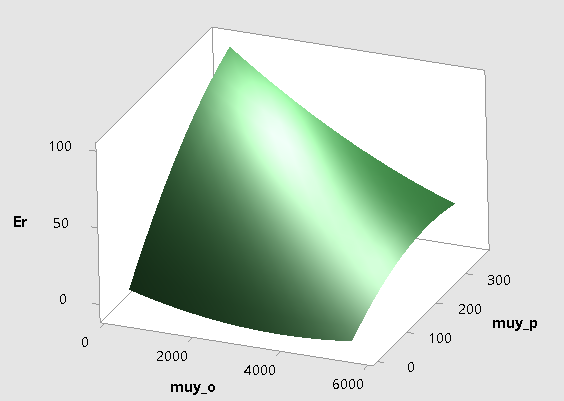
\includegraphics[scale=1]{Fig/SurfaceplotErfull.PNG}
		\caption{Đồ thị bề mặt của độ nhớt dầu, độ nhớt polymer và lượng dầu thu hồi tăng cường}
	\end{figure}
	\newline
	Độ tin cậy khi thực hiện xây dựng mô hình tối ưu cho cả 29 mẫu thí nghiệm chỉ đạt mức 77.92\% là tương đối thấp. Do đó không mang lại nhiều giá trị tính toán trong thực tế.
	\newpage
	\noindent
	Sau khi loại bỏ những thông số gây nhiễu, các giá trị đo được từ các mẫu dầu có độ nhớt nhỏ hơn 2000 mPa.s được đưa vào triển khai hàm tối ưu. Phương trình (16) chính là hàm mục tiêu được xây dựng cho các mẫu dầu có độ nhớt nhỏ hơn 2000 mPa.s (Dữ liệu được lấy từ Bảng 10, 11, 12, Phụ lục A. Mô hình hồi quy được thể hiện trong Phụ lục C):
	\begin{equation}
		E_r=-0.27+0.0033\mu_o+1.059\mu_p-0.000008\mu_o^2-0.00525\mu_p^2-0.000172\mu_o\mu_p
	\end{equation}
Model Summary:
\begin{table}[h]
\begin{flushleft}
\label{my-label}
\begin{tabular}{rrrr}
S       & R-sq    & R-sq(Adj) & R-sq(Pred) \\
2.87184 & 82.21\% & 74.13\%   & 60.83\%    
\end{tabular}
\end{flushleft}
\end{table}
	\newline
	Mức độ tin cậy của mô hình mới đạt giá trị 82.21\%, thể hiện khả năng tính toán, áp dụng trong thực tế. Mô hình mới cũng thể hiện được mức độ phụ thuộc của lượng dầu thu hồi tăng cường với các giá trị độ nhớt rõ ràng hơn.
	\begin{figure}[h]
		\centering
		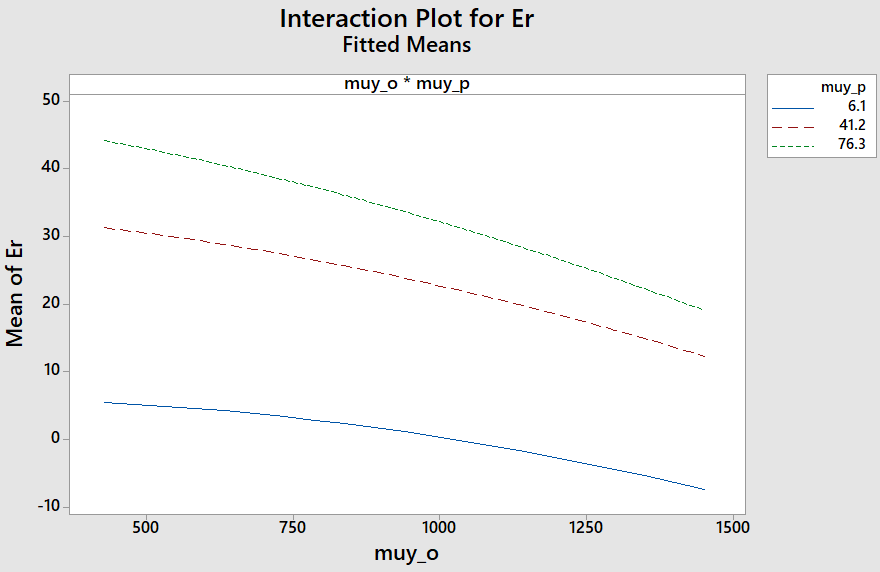
\includegraphics[scale=.7]{Fig/Effectcrossover.PNG}
		\caption{Ảnh hưởng của biến tương tác $\mu_o\mu_p$}
	\end{figure}
	\begin{figure}[h]
		\centering
		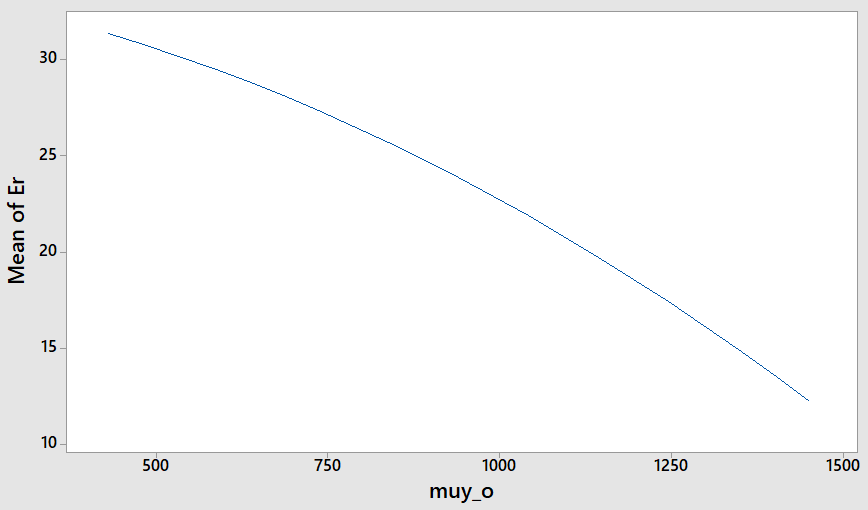
\includegraphics[scale=.7]{Fig/effectofmuyoil.PNG}
		\caption{Ảnh hưởng của biến độc lập $\mu_o$}
	\end{figure}
	\begin{figure}[h]
		\centering
		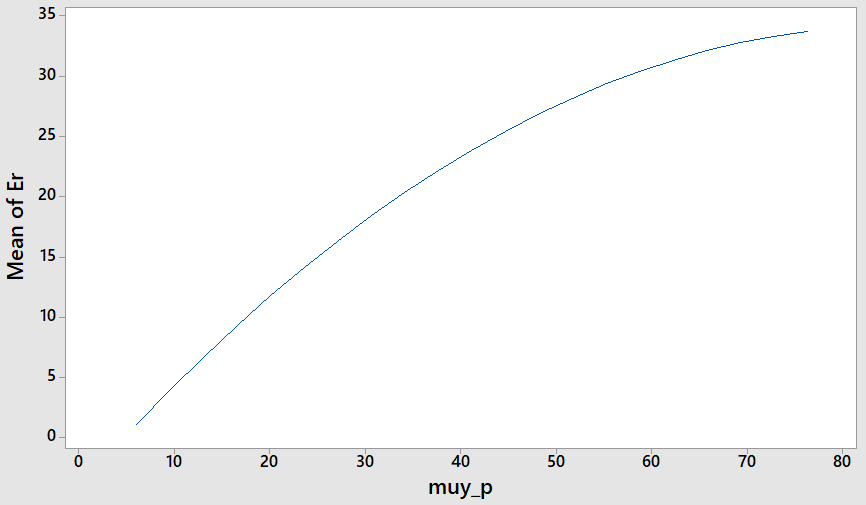
\includegraphics[scale=0.7]{Fig/effectofmuyp.PNG}
		\caption{Ảnh hưởng của biến độc lập $\mu_p$}
	\end{figure}
	\clearpage
	\subsection{Tỉ số độ linh động}
	Trong quá trình waterflood, tỉ số độ linh động \cite{chang1978polymer} được định nghĩa bằng phương trình (17):
		\begin{equation}
		M=\frac{k_w}{\mu_w}/\frac{k_{o}}{\mu_o}=\frac{k_{rw}}{\mu_{w}}/\frac{k_{ro}}{\mu_o}
		\end{equation}
	Giá trị này thể hiện tỉ số độ linh động trước khi breakthrough (nước bơm ép bắt đầu tràn vào phạm vi khai thác của giếng khai thác). Mặc dù quá trình polymer flooding đem lại nhiều hiệu quả nhưng thường chỉ được thực hiện sau khi breakthrough, vì vậy tỉ số độ linh động trong quá trình bơm ép polymer \cite{chang1978polymer} được tính theo công thức sau:
		\begin{equation}
			M=\frac{\lambda_{rp}}{\lambda_T}=\left(\frac{k_{rp}}{\mu_p}\right)/\left(\frac{k_{ro}}{\mu_o}+\frac{k_{rw}}{\mu_w}\right)
		\end{equation}
	Với $\lambda_{rp}$, $\lambda_T$ tương ứng là độ linh động tương đối của polymer và tổng độ linh động tương đối của dầu-nước. Những thông số này được đo đạt riêng lẻ với mô hình sandpack một chiều.\\
	Hình 21 thể hiện giá trị độ nhớt polymer tối ưu được dự đoán bằng phương trình hàm (16) khi giá trị thu hồi dầu tăng cường mong muốn là 19\% và giá trị độ nhớt dầu xấp xỉ 1327.5 mPa.s:
	\begin{figure}[h]
		\centering
		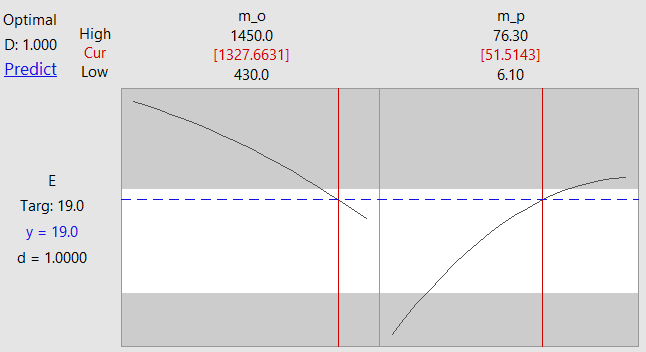
\includegraphics[scale=.9]{Fig/OptimizationPlot19.png}
		\caption{Độ nhớt tối ưu của polymer khi $E_r=19\%$}
	\end{figure}
\newpage
\noindent
	Lúc này giá trị tỉ số độ linh động sẽ được tính dựa vào công thức (18). Các giá trị độ thấm tương đối được đo trực tiếp từ mẫu dầu có độ nhớt xấp xỉ 1327.5 mPa.s, dung dịch polymer có độ nhớt 51.5 mPa.s và nước có độ nhớt 1.15 mPa.s như Bảng 8.
\begin{table}[h]
\centering
\caption{Giá trị độ thấm tương đối}
\label{my-label}
\begin{tabularx}{\textwidth}{@{}XXXX@{}}
\toprule
      & Oil  & Polymer & Water  \\ \midrule
$k_r (mD)$ & 0.87 & 0.44    & 0.0077 \\ \bottomrule
\end{tabularx}
\end{table}
\newline
	Giá trị tỉ số độ linh động:
	\begin{center}
	\centering
		$M=\left(\frac{0.44}{51.5}\right)/\left(\frac{0.87}{1327.5}+\frac{0.0077}{1.15}\right)=1.16$
	\end{center}
	Có thể thấy rõ giá trị tỉ số độ linh động gần như đạt mức tốt nhất.\\
	Hình 22 thể hiện giá trị độ nhớt tối ưu khi lượng dầu thu hồi tăng cường đạt mức lớn nhất (xấp xỉ 44\%) và giá trị độ nhớt dầu xấp xỉ 446 mPa.s.
	Các giá trị độ thấm tương ứng vẫn tiếp tục được đo trực tiếp đối với các mẫu dầu, nước và polymer tương ứng như Bảng 9:
\begin{table}[h]
\centering
\caption{Giá trị độ thấm tương đối}
\label{my-label}
\begin{tabularx}{\textwidth}{@{}XXXX@{}}
\toprule
      & Oil  & Polymer & Water  \\ \midrule
$k_r (mD)$ & 0.95 & 0.43    & 0.0013 \\ \bottomrule
\end{tabularx}
\end{table}	
\newline
	Giá trị tỉ số độ linh động:
	\begin{center}
	\centering
		$M=\left(\frac{0.43}{76.3}\right)/\left(\frac{0.95}{446}+\frac{0.0013}{1.15}\right)=1.73$
	\end{center}
	\begin{figure}[h]
		\centering
		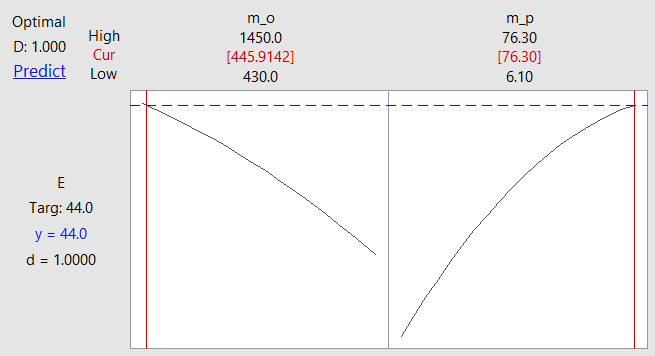
\includegraphics[scale=.9]{Fig/MaximumEr.PNG}
		\caption{Độ nhớt tối ưu của polymer khi $E_r$ lớn nhất}
	\end{figure}
	\noindent
	Lượng dầu thu hồi tăng cường và các giá trị tối ưu tương ứng được thể hiện như trong đồ thị\\ Hình 23:
	\begin{figure}[h]
		\centering
		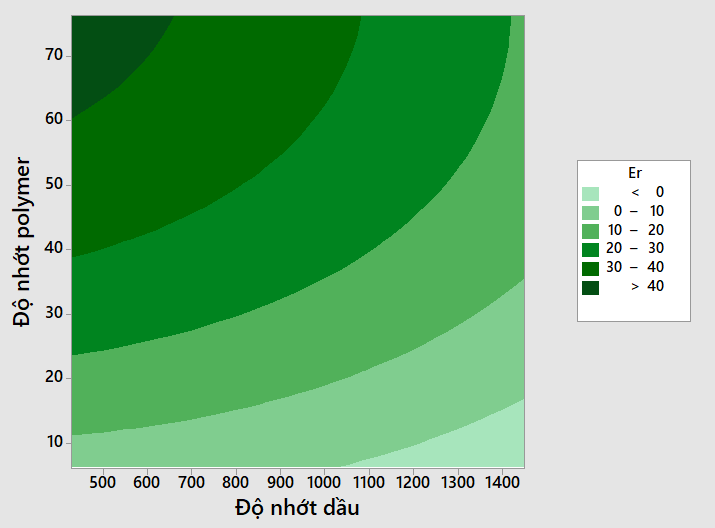
\includegraphics[scale=.8]{Fig/ContourEr.PNG}
		\caption{Đồ thị vòng của $E_r$ với độ nhớt dầu và độ nhớt polymer}
	\end{figure}
\clearpage
\noindent
\textbf{\LARGE Kết luận và kiến nghị}\\[-0.3cm]
\addcontentsline{toc}{section}{Kết luận và kiến nghị}
\newline
	Phương pháp bơm ép polymer là một trong những phương pháp thu hồi dầu tăng cường mang lại hiệu suất cao nhất khi được áp dụng cho thu hồi dầu có độ nhớt cao. Hai loại polymer được sử dụng nhiều nhất là Hydrolyzed Polyacrylamides (HPAM) và Xanthan.\\
	Sandpack flood test mang lại nhiều hiệu quả trong việc tiềm kiếm, xây dựng mối quan hệ tương quan giữa tỉ số độ linh động với độ nhớt của dầu và độ nhớt của polymer. Dựa vào các dữ liệu từ thí nghiệm sandpack-flood, hàm tối ưu lượng dầu thu hồi tăng cường phụ thuộc vào độ nhớt dầu và độ nhớt polymer được xây dựng với độ tin cậy 82.21\%.
	\begin{center}
	\centering
		$E_r=-0.27+0.0033\mu_o+1.059\mu_p-0.000008\mu_o^2-0.00525\mu_p^2-0.000172\mu_o\mu_p$
	\end{center}
	Giá trị tỉ số độ linh động tính toán thông qua hàm tối ưu nằm trong khoảng từ 1.16 đến 1.73 được coi là tốt nhất, mang lại lượng dầu thu hồi tăng cường cao nhất khi sử dụng phương pháp bơm ép polymer.\\
	Đối với dầu có độ nhớt trên 2000 mPa.s, quá trình thực hiện bơm ép polymer phải sử dụng dung dịch có độ nhớt từ 250 mPa.s mới có thể đem hiệu quả về lượng dầu thu hồi tăng cường. Tuy nhiên, khi sử dụng dung dịch polymer có độ nhớt quá lớn sẽ không mang lại nhiều hiệu quả về kinh tế do chi phí thực hiện quá cao. Ngược lại, nếu độ nhớt dung dịch polymer quá nhỏ sẽ không cho hiệu quả về khai thác.\\
	Tuy nhiên, mô hình sandpack cũng có nhiều nhược điểm. Trong đó, nhược điểm đáng chú ý nhất là không tạo ra được môi trường rỗng sát với thực tế, dẫn đến khi đo đạt độ thấm tương đối của polymer sẽ mang nhiều sai sót, làm giảm mức độ tin cậy của hàm mục tiêu. Quá trình đo cần phải thực hiện nhiều lần để tăng mức độ tin cậy của mô hình trong khi áp dụng vào thực tế.\\
	Qua quá trình hoàn thiện đồ án, nhóm tác giả nhận thấy độ nhớt dầu và độ nhớt polymer mặc dù là hai yếu tố chính tác động lên tỉ số độ linh động nhưng chưa hoàn toàn quyết định được mức độ hiệu quả chính thức. Những yếu tố khác như nhiệt độ, áp suất, khả năng kéo dài thời gian ổn định trong vỉa đồng thời cũng tác động đến hiệu suất thu hồi dầu. Tuy nhiên, điều kiện hiện tại chưa cho phép nhóm thực hiện nghiên cứu rộng sang những yếu tố nêu trên. Do đó, nhằm mục đích hoàn thiện đồ án nhóm tác giả mong muốn trong tương lai, những nghiên cứu về tối ưu lượng dầu thu hồi hay nâng cao tối đa chỉ số thu hồi dầu cần được thực hiện nhiều hơn và cần đặc biệt quan tâm đến những yếu tố đã bỏ sót trong đồ án này.
	\newpage

\addcontentsline{toc}{section}{Tài liệu tham khảo}
\bibliographystyle{ieeetr}
\bibliography{ref}

	\clearpage
	\noindent
\textit{\textbf{\LARGE Phụ Lục A}}\\
\addcontentsline{toc}{section}{Phụ Lục A}
Kết quả thu được sau thí nghiệm với 29 mẫu sandpack-column.
\begin{table}[h]
\centering
\caption{Dầu có độ nhớt 430 mPa.s}
\label{my-label}
\begin{tabularx}{\textwidth}{@{}XX|XXX|XXXX|X@{}}
\toprule
\multicolumn{2}{c}{Sandpack} & \multicolumn{3}{c}{Waterflood} & \multicolumn{4}{c}{Polymer flooding} & $E_t$ \\ \midrule
No.        & $S_{iw}$        & PV      & E    & $\mu_w$   & OOIP   & $\mu_p$  & $E_r$ & $k_{rp}$ &       \\
1          & 0.112           & 3.5     & 41.9     & 1.15      & 3.1    & 6.1      & 2.2   & 0.78     & 44.1  \\
2          & 0.109           & 4       & 42.4     & 1.15      & 3.56   & 8.5      & 4.9   & 0.76     & 47.3  \\
3          & 0.125           & 3.2     & 41.8     & 1.15      & 2.8    & 10.7     & 14.6  & 0.74     & 56.4  \\
4          & 0.133           & 2.8     & 40.2     & 1.15      & 2.43   & 15.2     & 15.7  & 0.72     & 55.9  \\
5          & 0.135           & 2.8     & 40.2     & 1.15      & 2.4    & 21.8     & 17.5  & 0.69     & 57.7  \\ \bottomrule
\end{tabularx}
\end{table}
\begin{table}[h]
\centering
\caption{Dầu có độ nhớt 1108 mPa.s}
\label{my-label}
\begin{tabularx}{\textwidth}{@{}XX|XXX|XXXX|X@{}}
\toprule
\multicolumn{2}{c}{Sandpack} & \multicolumn{3}{c}{Waterflood} & \multicolumn{4}{c}{Polymer flooding} & $E_t$ \\ \midrule
No.        & $S_{iw}$        & PV      & E    & $\mu_w$   & OOIP   & $\mu_p$  & $E_r$ & $k_{rp}$ &       \\
1          & 0.092            & 4.5     & 40.3     & 1.15      & 4.1    & 14.6     & 3.9   & 0.74     & 44.2  \\
2          & 0.106           & 5.3     & 42.2     & 1.15      & 4.73   & 15.6     & 4.4   & 0.71     & 46.6  \\
3          & 0.133           & 5       & 41.9     & 1.15      & 4.34   & 18.5     & 10    & 0.70     & 51.9  \\
4          & 0.112           & 5.2     & 42       & 1.15      & 4.62   & 21.8     & 10.5  & 0.69     & 52.5  \\
5          & 0.11            & 5.1     & 41.8     & 1.15      & 4.54   & 29.3     & 12    & 0.66     & 53.8  \\
6          & 0.108           & 4.8     & 41.5     & 1.15      & 4.28   & 35.4     & 14.5  & 0.61     & 56    \\
7          & 0.105           & 5.2     & 42       & 1.15      & 4.65   & 37.6     & 15.6  & 0.57     & 57.6  \\ \bottomrule
\end{tabularx}
\end{table}
\begin{table}[h]
\centering
\caption{Dầu có độ nhớt 1450 mPa.s}
\label{my-label}
\begin{tabularx}{\textwidth}{@{}XX|XXX|XXXX|X@{}}
\toprule
\multicolumn{2}{c}{Sandpack} & \multicolumn{3}{c}{Waterflood} & \multicolumn{4}{c}{Polymer flooding} & $E_t$ \\ \midrule
No.        & $S_{iw}$        & PV      & E    & $\mu_w$   & OOIP   & $\mu_p$  & $E_r$ & $k_{rp}$ &       \\
1          & 0.107           & 9.6     & 42.7     & 1.15      & 8.57   & 27.7     & 4.1   & 0.58     & 46.8  \\
2          & 0.111           & 10.8    & 42.2     & 1.15      & 9.6    & 29.3     & 5.2   & 0.55     & 47.4  \\
3          & 0.86            & 10.1    & 42.5     & 1.15      & 9.23   & 38.4     & 14.3  & 0.50     & 56.8  \\
4          & 0.101           & 8       & 42.4     & 1.15      & 7.19   & 51.3     & 16.7  & 0.44     & 58.9  \\
5          & 0.109           & 8.8     & 41.9     & 1.15      & 7.84   & 76.3     & 19    & 0.41     & 60.9  \\ \bottomrule
\end{tabularx}
\end{table}
\begin{table}[h]
\centering
\caption{Dầu có độ nhớt 2900 mPa.s}
\label{my-label}
\begin{tabularx}{\textwidth}{@{}XX|XXX|XXXX|X@{}}
\toprule
\multicolumn{2}{c}{Sandpack} & \multicolumn{3}{c}{Waterflood} & \multicolumn{4}{c}{Polymer flooding} & $E_t$ \\ \midrule
No.        & $S_{iw}$        & PV      & E    & $\mu_w$   & OOIP   & $\mu_p$  & $E_r$ & $k_{rp}$ &       \\
1          & 0.11            & 10.6    & 40.9     & 1.15      & 9.43   & 35.3     & 2.8   & 0.49     & 43.7  \\
2          & 0.111           & 13.1    & 41       & 1.15      & 11.65  & 38.4     & 3.7   & 0.46     & 44.7  \\
3          & 0.119           & 14.2    & 40.4     & 1.15      & 12.51  & 51.8     & 13.5  & 0.44     & 53.9  \\
4          & 0.115           & 12.9    & 42.4     & 1.15      & 11.41  & 76.3     & 16.5  & 0.43     & 58.9  \\
5          & 0.125           & 11.8    & 41.5     & 1.15      & 10.32  & 93.2     & 18.4  & 0.41     & 58.9  \\ \bottomrule
\end{tabularx}
\end{table}
\begin{table}[h]
\centering
\caption{Dầu có độ nhớt 5500 mPa.s}
\label{my-label}
\begin{tabularx}{\textwidth}{@{}XX|XXX|XXXX|X@{}}
\toprule
\multicolumn{2}{c}{Sandpack} & \multicolumn{3}{c}{Waterflood} & \multicolumn{4}{c}{Polymer flooding} & $E_t$ \\ \midrule
No.        & $S_{iw}$        & PV      & E    & $\mu_w$   & OOIP   & $\mu_p$  & $E_r$ & $k_{rp}$ &       \\
1          & 0.107           & 13.8    & 41       & 1.15      & 12.32  & 40.1     & 2.8   & 0.47     & 43.8  \\
2          & 0.105           & 14.2    & 41.6     & 1.15      & 12.71  & 51.8     & 4.2   & 0.44     & 45.8  \\
3          & 0.102           & 14.5    & 41.4     & 1.15      & 13.02  & 112.5    & 17    & 0.37     & 58.4  \\
4          & 0.115           & 15      & 42.3     & 1.15      & 13.27  & 128.8    & 18.2  & 0.35      & 60.5  \\
5          & 0.105           & 15.4    & 42.6     & 1.15      & 13.78  & 193.2    & 18.7  & 0.31     & 61.3  \\
6          & 0.111           & 14      & 41.1     & 1.15      & 12.44  & 251.7    & 20.7  & 0.27     & 61.8  \\
7          & 0.107           & 17.1    & 42.1     & 1.15      & 15.27  & 359.3    & 21    & 0.24     & 63.1  \\ \bottomrule
\end{tabularx}
\end{table}
\clearpage
\noindent
\textit{\textbf{\LARGE Phụ Lục B}}\\
\addcontentsline{toc}{section}{Phụ Lục B}
\noindent
\textbf{Response Surface Regression:\\
Oil tertiary recovery versus oil viscosity and polymer viscosity}\\
\newline
\code{Analysis of Variance}\\
\newline
\code{Source}\hspace*{3cm}\code{DF}\hspace*{1cm}\code{Adj SS}\hspace*{1cm}\code{Adj MS}\hspace*{1cm}\code{F-Value}\hspace*{1cm}\code{P-Value}\\
\code{Model}\hspace*{3.5cm}\code{5}\hspace*{1cm}\code{901.90}\hspace*{1cm}\code{180.38}\hspace*{1.5cm}\code{16.23}\hspace*{1.4cm}\code{0.000}\\
\hspace*{0.5cm}\code{Linear}\hspace*{2.75cm}\code{2}\hspace*{1cm}\code{217.69}\hspace*{1cm}\code{108.85}\hspace*{1.75cm}\code{9.79}\hspace*{1.4cm}\code{0.001}\\
\hspace*{1cm}\code{muy o}\hspace*{2.5cm}\code{1}\hspace*{1cm}\code{145.69}\hspace*{1cm}\code{145.69}\hspace*{1.5cm}\code{13.11}\hspace*{1.4cm}\code{0.001}\\
\hspace*{1cm}\code{muy p}\hspace*{2.5cm}\code{1}\hspace*{1cm}\code{145.40}\hspace*{1cm}\code{190.40}\hspace*{1.5cm}\code{17.13}\hspace*{1.4cm}\code{0.001}\\
\hspace*{0.5cm}\code{Square}\hspace*{2.75cm}\code{2}\hspace*{1cm}\code{268.94}\hspace*{1cm}\code{134.47}\hspace*{1.5cm}\code{12.10}\hspace*{1.4cm}\code{0.000}\\
\hspace*{1cm}\code{muy o.muy o}\hspace*{1cm}\code{1}\hspace*{1.25cm}\code{89.29}\hspace*{1.25cm}\code{89.29}\hspace*{1.75cm}\code{8.04}\hspace*{1.4cm}\code{0.009}\\
\hspace*{1cm}\code{muy p.muy p}\hspace*{1cm}\code{1}\hspace*{1cm}\code{109.72}\hspace*{1cm}\code{109.72}\hspace*{1.75cm}\code{9.87}\hspace*{1.4cm}\code{0.005}\\
\hspace*{0.5cm}\code{2-Way Interaction}\hspace*{0.05cm}\code{1}\hspace*{1.25cm}\code{62.61}\hspace*{1.25cm}\code{62.61}\hspace*{1.75cm}\code{5.63}\hspace*{1.4cm}\code{0.026}\\
\hspace*{1cm}\code{muy o.muy p}\hspace*{1.01cm}\code{1}\hspace*{1.25cm}\code{62.61}\hspace*{1.25cm}\code{62.61}\hspace*{1.75cm}\code{5.63}\hspace*{1.4cm}\code{0.026}\\
\code{Error}\hspace*{3.25cm}\code{23}\hspace*{1cm}\code{255.60}\hspace*{1.25cm}\code{11.11}\\
\code{Total}\hspace*{3.26cm}\code{28}\hspace*{0.755cm}\code{1157.49}\\
\newline
\code{Model Summary}\\
\hspace*{2cm}\code{S}\hspace*{1.5cm}\code{R-sq}\hspace*{1.5cm}\code{R-sq(adj)}\hspace*{1.5cm}\code{R-sq(Pred)}\\
\hspace*{0.49cm}\code{3.33359}\hspace*{1cm}\code{77.92\%}\hspace*{2.15cm}\code{73.12\%}\hspace*{2.5cm}\code{29.10\%}\newpage
\noindent
\code{Coded Coefficients}\\
\code{Term}\hspace*{3cm}\code{Coef}\hspace*{1cm}\code{SE Coef}\hspace*{1cm}\code{T-Value}\hspace*{1cm}\code{P-Value}\hspace*{1cm}\code{VIF}\\
\code{Constant}\hspace*{1.8cm}\code{35.61}\hspace*{1.7cm}\code{4.04}\hspace*{1.7cm}\code{8.82}\hspace*{1.4cm}\code{0.000}\hspace*{1.5cm}\\
\code{muy o}\hspace*{2.3cm}\code{-22.50}\hspace*{1.7cm}\code{6.21}\hspace*{1.45cm}\code{-3.62}\hspace*{1.4cm}\code{0.001}\hspace*{0.5cm}\code{55.61}\\
\code{muy p}\hspace*{2.55cm}\code{28.32}\hspace*{1.7cm}\code{6.84}\hspace*{1.7cm}\code{4.14}\hspace*{1.4cm}\code{0.000}\hspace*{0.5cm}\code{23.93}\\
\code{muy o.muy o}\hspace*{1.3cm}\code{7.35}\hspace*{1.7cm}\code{2.59}\hspace*{1.7cm}\code{2.83}\hspace*{1.4cm}\code{0.009}\hspace*{0.75cm}\code{2.47}\\
\code{muy p.muy p}\hspace*{0.8cm}\code{-11.86}\hspace*{1.7cm}\code{3.77}\hspace*{1.45cm}\code{-3.14}\hspace*{1.4cm}\code{0.005}\hspace*{1.5cm}\code{3}\\
\code{muy o.muy p}\hspace*{0.8cm}\code{-17.23}\hspace*{1.7cm}\code{7.26}\hspace*{1.45cm}\code{-2.37}\hspace*{1.4cm}\code{0.026}\hspace*{0.5cm}\code{33.63}\\
\newline
\code{Regression Equation in Uncoded Units}\\
\newline
\code{E = 9.15 - 0.00863muy o + 0.4134muy p + 0.000001muy o.muy o \\ \hspace*{4cm}- 0.00038muy p.muy p - 0.000038muy o.muy p}\\
\newline
\code{Fits and Diagnostics for Unusual Observations}\\
\newline
\code{Obs}\hspace*{2cm}\code{E}\hspace*{1.5cm}\code{Fit}\hspace*{1.5cm}\code{Resid}\hspace*{1.5cm}\code{Std Resid}\\
\hspace*{0.25cm}\code{17}\hspace*{1cm}\code{19.00}\hspace*{1cm}\code{24.11}\hspace*{1.5cm}\code{-5.11}\hspace*{2.5cm}\code{-2.11}\hspace{1cm}\code{R}\\
\hspace*{0.25cm}\code{19}\hspace*{1cm}\code{21.00}\hspace*{1cm}\code{19.69}\hspace*{1.75cm}\code{1.31}\hspace*{2.75cm}\code{1.54}\hspace{1cm}\code{X}\\
\code{R: Large residual}\\
\code{X: Unsual X}


\newpage
\noindent
\textit{\textbf{\LARGE Phụ Lục C}}\\
\addcontentsline{toc}{section}{Phụ Lục C}
\noindent
\textbf{Response Surface Regression:\\
Oil tertiary recovery versus oil viscosity and polymer viscosity}\\
\newline
\code{Analysis of Variance}\\
\newline
\code{Source}\hspace*{3cm}\code{DF}\hspace*{1cm}\code{Adj SS}\hspace*{1cm}\code{Adj MS}\hspace*{1cm}\code{F-Value}\hspace*{1cm}\code{P-Value}\\
\code{Model}\hspace*{3.5cm}\code{5}\hspace*{1cm}\code{419.28}\hspace*{1cm}\code{083.86}\hspace*{1.5cm}\code{10.17}\hspace*{1.4cm}\code{0.001}\\
\hspace*{0.5cm}\code{Linear}\hspace*{2.75cm}\code{2}\hspace*{1cm}\code{134.50}\hspace*{1cm}\code{067.25}\hspace*{1.75cm}\code{8.15}\hspace*{1.4cm}\code{0.007}\\
\hspace*{1cm}\code{muy o}\hspace*{2.5cm}\code{1}\hspace*{1cm}\code{043.28}\hspace*{1cm}\code{043.28}\hspace*{1.5cm}\code{05.25}\hspace*{1.4cm}\code{0.007}\\
\hspace*{1cm}\code{muy p}\hspace*{2.5cm}\code{1}\hspace*{1cm}\code{083.15}\hspace*{1cm}\code{083.15}\hspace*{1.5cm}\code{10.08}\hspace*{1.4cm}\code{0.009}\\
\hspace*{0.5cm}\code{Square}\hspace*{2.75cm}\code{2}\hspace*{1cm}\code{018.97}\hspace*{1cm}\code{009.49}\hspace*{1.5cm}\code{01.15}\hspace*{1.4cm}\code{0.352}\\
\hspace*{1cm}\code{muy o.muy o}\hspace*{1cm}\code{1}\hspace*{1.25cm}\code{03.98}\hspace*{1.25cm}\code{03.98}\hspace*{1.75cm}\code{0.48}\hspace*{1.4cm}\code{0.502}\\
\hspace*{1cm}\code{muy p.muy p}\hspace*{1cm}\code{1}\hspace*{1cm}\code{018.85}\hspace*{1cm}\code{018.85}\hspace*{1.75cm}\code{2.29}\hspace*{1.4cm}\code{0.159}\\
\hspace*{0.5cm}\code{2-Way Interaction}\hspace*{0.05cm}\code{1}\hspace*{1.25cm}\code{01.67}\hspace*{1.25cm}\code{01.67}\hspace*{1.75cm}\code{0.20}\hspace*{1.4cm}\code{0.662}\\
\hspace*{1cm}\code{muy o.muy p}\hspace*{1.01cm}\code{1}\hspace*{1.25cm}\code{01.67}\hspace*{1.25cm}\code{01.67}\hspace*{1.75cm}\code{0.20}\hspace*{1.4cm}\code{0.662}\\
\code{Error}\hspace*{3.25cm}\code{11}\hspace*{1cm}\code{090.72}\hspace*{1.25cm}\code{08.23}\\
\code{Total}\hspace*{3.26cm}\code{16}\hspace*{0.755cm}\code{0510.00}\\
\newline
\code{Model Summary}\\
\hspace*{2cm}\code{S}\hspace*{1.5cm}\code{R-sq}\hspace*{1.5cm}\code{R-sq(adj)}\hspace*{1.5cm}\code{R-sq(Pred)}\\
\hspace*{0.49cm}\code{2.87184}\hspace*{1cm}\code{82.21\%}\hspace*{2.15cm}\code{74.14\%}\hspace*{2.5cm}\code{60.83\%}\newpage
\noindent
\code{Coded Coefficients}\\
\code{Term}\hspace*{3cm}\code{Coef}\hspace*{1cm}\code{SE Coef}\hspace*{1cm}\code{T-Value}\hspace*{1cm}\code{P-Value}\hspace*{1cm}\code{VIF}\\
\code{Constant}\hspace*{1.8cm}\code{23.89}\hspace*{1.7cm}\code{2.73}\hspace*{1.7cm}\code{8.76}\hspace*{1.4cm}\code{0.000}\hspace*{1.5cm}\\
\code{muy o}\hspace*{2.3cm}\code{-09.52}\hspace*{1.7cm}\code{4.16}\hspace*{1.45cm}\code{-2.29}\hspace*{1.4cm}\code{0.043}\hspace*{0.5cm}\code{22.87}\\
\code{muy p}\hspace*{2.55cm}\code{16.30}\hspace*{1.7cm}\code{5.13}\hspace*{1.7cm}\code{3.18}\hspace*{1.4cm}\code{0.009}\hspace*{0.5cm}\code{12.88}\\
\code{muy o.muy o}\hspace*{1.05cm}\code{-2.06}\hspace*{1.7cm}\code{2.97}\hspace*{1.45cm}\code{-0.69}\hspace*{1.4cm}\code{0.502}\hspace*{0.75cm}\code{2.66}\\
\code{muy p.muy p}\hspace*{0.8cm}\code{-06.47}\hspace*{1.7cm}\code{4.28}\hspace*{1.45cm}\code{-1.51}\hspace*{1.4cm}\code{0.159}\hspace*{0.75cm}\code{4.26}\\
\code{muy o.muy p}\hspace*{0.8cm}\code{-03.08}\hspace*{1.7cm}\code{6.85}\hspace*{1.45cm}\code{-0.45}\hspace*{1.4cm}\code{0.662}\hspace*{0.5cm}\code{25.95}\\
\newline
\code{Regression Equation in Uncoded Units}\\
\newline
\code{E = -0.27 - 0.0033muy o + 1.059muy p + 0.000008muy o.muy o \\ \hspace*{4cm}- 0.00525muy p.muy p - 0.000172muy o.muy p}\\
%\addcontentsline{toc}{section}{Tài liệu tham khảo}
%\bibliographystyle{ieeetr}
%\bibliography{ref}
\end{document}